
\setcounter{section}{0}
\renewcommand\thefigure{\arabic{chapter}.\arabic{figure}}
\renewcommand\thetable{\arabic{chapter}.\arabic{table}}
\renewcommand\thesubsection{\arabic{chapter}.\arabic{section}.\arabic{subsection}}
\renewcommand\thesection{\arabic{chapter}.\arabic{section}}
\setcounter{figure}{0}
\setcounter{table}{0}

\section{Probing the Infant Universe}\label{sec:intro_joint}

As discussed, the infant Universe, corresponding to cosmic time between 200 and 700 million years after the Big Bang, remains largely unexplored. This epoch is traced by some of the most remarkable events in cosmic history, such as the birth of primordial stars, formation of the very first black holes and assembly of early galaxies. The nature of the first bright objects to form and the exact timing of these events are yet to be constrained by observations. Theoretical studies and numerical simulations suggest that first stars form between $z\sim 20-60$, i.e. around $35-200$ million years after the Big Bang\cite{Bond_pop3_1981, Bromm_pop3_2004, Klessen2019}, and, thus, are currently out of reach of the modern telescopes like JWST. 

Although the controversial EDGES signal is the only detection of the high-redshift 21-cm signal reported to date, advances have been made by other existing radio telescopes, as alluded to in the introduction, with upper limits reported by both the interferometers such as PAPER \citep[Precision Array for Probing the Epoch of Reionization, ][]{Jacobs_Paper_limits_2015}, MWA \cite{Trott_mwa_2020, Kolopanis_MWA_limits_2022}, LOFAR \cite{Patil_2017, Mertens_2020}, AARTFAAC \citep[Amsterdam-ASTRON Radio Transients Facility And Analysis Center, ][]{AARTFAAC_2020} and HERA \cite{HERA_2022a, HERA_2022b, HERA_2022c} on the 21-cm power spectrum, which quantifies the variation in the 21-cm brightness field as a function of angular scale and time, and on the global  21-cm signal by SARAS \citep[][e.g. the previous two chapters]{Singh_saras2_2017, Singh_saras2_2018, Bevins_SARAS2_2022, Bevins_saras3_2022}, EDGES High Band \cite{Monsalve_EDGES_HB_1_2017, Monsalve_EDGES_HB_2_2018, Monsalve_EDGES_HB_3_2019} and LEDA \cite{Bernardi_LEDA_2016}. These upper limits are becoming increasingly constraining and have already being used to put limits on the  properties of high-redshift luminous objects \cite{Mondal_LOFAR_2020, HERA_2022b, HERA_2022c, Singh_saras2_2017, Singh_saras2_2018, Bevins_SARAS2_2022, Bevins_saras3_2022}. The ongoing and upcoming experiments including SARAS \cite{SARAS3}, MIST \cite{MIST}, REACH \cite{de_lera_acedo_reach_2022}, LOFAR \cite{LOFAR_current_EoR_2018}, NenuFAR \citep[ New Extension in Nançay Upgrading loFAR,][]{Zarka_nenuFar_2018}, HERA \cite{HERA_2017}, the SKA and future proposed space based missions such as DAPPER and FARSIDE \cite{Burns_Moon_2021} aim to further improve our understanding of the infant Universe.

Existing upper limits on the 21-cm signal provide the first very weak constraints on the astrophysical sources at a broad range of redshifts. 
In this chapter, we take the current tightest publicly available upper limits from the HERA interferometer on the magnitude of the 21-cm power spectrum at redshifts $z \approx 8$ and $\approx 10$  which provides a window to the EoR when ultraviolet photons emitted by first massive galaxies efficiently ionize the neutral hydrogen gas \cite{HERA_2022b}, and the SARAS3 radiometer \cite{SARAS3} that  probes the sky-averaged 21-cm emission at higher redshifts between $z\approx 15 - 25$ when the first stars and X-ray emitting objects are expected to have formed in small galaxies during the Cosmic Dawn. We combine these two data sets for the first time to improve constraints on the properties of the first galaxies and the state of the neutral gas. We develop the methods to perform the joint analysis using a machine learning enhanced Bayesian workflow and pave the way for future discoveries. We find that when considered together, these two experiments provide a better leverage on theoretical scenarios that bridge across the wide redshift range compared to the constraints from each individual experiment. In synergy, the two experiments leave  only $64.9^{+0.3}_{-0.1}$\% of the explored broad theoretical parameter space to be consistent with the joint data set, in comparison to $92.3^{+0.3}_{-0.1}$\% for SARAS3 and $79.0^{+0.5}_{-0.2}$\% for HERA alone. We use the joint analysis to limit  star formation efficiency, minimum halo mass for star formation, X-ray luminosity of early emitters and the radio luminosity of early galaxies. The joint analysis disfavours at 68\% confidence a combination of galaxies with X-ray emission that is $\lesssim 33$ and radio emission that is $\gtrsim 32$ times as efficient as present day galaxies.

In \cref{sec:method_joint} we review the data and the specifics of the experiments incorporated in our analysis. This is followed by a discussion about the synergies between the power spectrum and sky-averaged 21-cm experiments in the same section. We present the implications of our work for the astrophysical constraints and the validity of the EDGES absorption feature as a sky-averaged 21-cm signal in \cref{sec:results_joint}. This is followed by a summary in \cref{sec:conclusions_joint}. Additional information about the methodology and additional results can be found in \cref{sec:suplimentary_joint}.


\Cref{sec:power_spec_emulation} and \cref{sec:igm_temperature_emulation} were led by Stefan Heimersheim for \cite{Bevins_hera_saras3_2023} and similarly the work in \cref{sec:other_interferometers} was led by Irene Abril-Cabezas. The co-authors, Stefan Heimersheim, Irene Abril-Cabezas, Anastasia Fialkov, Eloy de Lera Acedo, Will Handley, Saurabh Singh and Rennan Barkana, of \cite{Bevins_hera_saras3_2023} provided comments on the manuscript that this chapter is based on.

\section{Methodology} \label{sec:method_joint}

The third iteration of the SARAS radiometer experiment took 15 hours of data, integrated in the frequency range $55 - 85$ MHz, from a lake in Southern India. After corrections were made for the receiver noise temperature, radio frequency interference and emission from the water beneath the antenna, the data was appropriately scaled by the total efficiency of the system to produce a measurement of the average sky temperature which is expected to include the Galactic and extra-galactic foregrounds as well as the 21-cm signal. SARAS3 reported a null detection of the EDGES absorption feature with a confidence of 95.3\% \cite{SARAS3} and more recently the data has been used to place constraints on the properties of the first galaxies which we discuss in more detail below \citep[\cref{ch:saras3},][]{Bevins_saras3_2022}.

SARAS2, the previous iteration of the instrumentation, recorded data at higher frequencies~(lower redshifts) of $110 - 200$~MHz and was found to contain a non-smooth systematic structure possibly caused by emission from the ground that the antenna was placed on. The data has been used to derive constraints on galaxies in the infant Universe, initially by fitting the foreground and systematic structure together with high order polynomials \cite{Singh_saras2_2017, Singh_saras2_2018} and subsequently by modelling the two components separately \citep[\cref{ch:saras2},][]{Bevins_SARAS2_2022}. In \cref{sec:suplimentary_joint} we combine constraints from the latter with constraints from SARAS3 and HERA.

To date, interferometric experiments have only observed upper limits of the cosmological 21-cm power spectrum, which still allow for a large range of realistic astrophysical scenarios. The tightest constraints are derived from the data from the HERA interferometer \cite{HERA_2022a}, followed by MWA in the redshift range $z = 6.5 - 8.7$ \cite{Trott_mwa_2020} and LOFAR, which provide the tightest upper limits at redshifts $z \sim 9.1$ \cite{Patil_2017} and $z \sim 9.3 - 10.6$ \cite{Mertens_2020}. The HERA telescope is a radio interferometer located in the Karoo Desert of South Africa \cite{HERA_2017} and has conducted its first observing campaign from 2017 to 2018. Already, this first public data release delivered the strongest constraints on the 21-cm power spectrum to date. The publicly available HERA data\footnote{Note that an analysis of Internal Data Release 3~(IDR3) was recently published \cite{HERA_2022c} which, at the time of writing, is not publicly available. IDR3 included the data used to arrive at the earlier limits on the power spectrum\cite{HERA_2022b} used here, along with an additional 76 nights of observations. Analysis of the data on the class of models explored in this work showed led to only a small improvement in the astrophysical constraints.} from the analysis of Internal Data Release 2 that we use in this chapter is based on 18 nights of observations, with 39 antennas operating at science quality level. For our analysis, we employ the publicly available spherically averaged power spectra derived from this data \cite{HERA_2022a}, in the wavenumber range $k=0.128\,h\mathrm{Mpc}^{-1}$ to $0.960\,h\mathrm{Mpc}^{-1}$ and from the two bands focusing on redshifts $z=7.9$ and $10.3$. In \cref{sec:suplimentary_joint} we consider the implications of including the upper limits on the power spectrum from MWA and LOFAR in our joint analysis.
 
In 21-cm cosmology, data analysis efforts are increasingly employing Bayes theorem 
\begin{equation}
    \mathcal{P}(\theta|D, \mathcal{M}) = \frac{\mathcal{L}(\theta) \pi(\theta)}{\mathcal{Z}},
    \label{eq:bayes}
\end{equation}
to derive constraints on the astrophysical scenarios of the early Universe. To recap, the likelihood, $\mathcal{L}(\theta)$, represents the probability that we observe the data, $D$, from SARAS3 or HERA given a particular model, $\mathcal{M}$. The prior, $\pi(\theta)$, represents our assumed knowledge before we consider any data and the evidence, $\mathcal{Z}$, is a normalisation constant.
The posterior, $\mathcal{P}(\theta|D, \mathcal{M})$, tells us which parts of the parameter space, $\theta$, given the data and chosen model, are more probable than others. The evaluation of Bayes theorem is usually performed with Nested Sampling or Markov Chain Monte Carlo~(MCMC) algorithms (see \cref{sec:suplimentary_joint}). In many 21-cm experiments, $\theta$ is composed of parameters that describe instrumental effects, $\theta_{I}$, foregrounds, $\theta_{fg}$, and the astrophysical processes that influence the 21-cm signal, $\theta_{21}$. We typically refer to the set of $\theta_{I}$ and $\theta_{fg}$ as the nuisance parameters $\alpha$. Since we are only interested in the 21-cm signal, we have to approximate the marginal or nuisance-free posterior $\mathcal{P}(\theta_{21}|D, \mathcal{M})$ given samples on $\mathcal{P}(\theta|D, \mathcal{M})$. We can do this with normalising flows and the marginal Bayesian statistics code \textsc{margarine} \cite{margarine_neurips, margarine_maxent}. The code is described in \cref{ch:margarine}, in summary it allows us to calculate the marginal posterior and in turn the nuisance-free likelihood, $\mathcal{L}(\theta_{21})$, for HERA and SARAS3 for a given set of parameters via a trained density estimator. Since the experiments are independent, we can subsequently multiply the two likelihoods together to produce a joint likelihood
\begin{equation}
    \mathcal{L}_{\textnormal{joint}}(\theta_{21}) = \mathcal{L}_{\textnormal{HERA}}(\theta_{21})~\mathcal{L}_{\textnormal{SARAS3}}(\theta_{21}),
\end{equation}
and sample this in \cref{eq:bayes} in a subsequent Nested Sampling or MCMC run to produce joint constraints on early astrophysics
We recap the astrophysical processes included in the modelling,  and the definition of $\theta_{21}$, next.

In order to realistically model the range of time covered by the Cosmic Dawn and Epoch of Reionization, we need a consistent modelling of the cosmological and astrophysical processes from redshift 60, when star formation might have begun, all the way to redshift 5 at the end of the EoR. To that end we employ semi-numerical simulations \cite{Visbal_2012,Fialkov_lyw_2013, fialkov_observable_2014, Fialkov_rich_2014, Reis_sta_2021} that have previously been used in this thesis to analysis data from SARAS2 \cite{Bevins_SARAS2_2022} and SARAS3 \cite{Bevins_saras3_2022} as well as to analyse data from HERA \cite{HERA_2022b}, LOFAR \cite{Mondal_LOFAR_2020} and EDGES High-Band \cite{Monsalve_EDGES_HB_3_2019} data. We model the three-dimensional 21-cm field as a function of cosmic time during the infant Universe taking into account important astrophysical process including the Wouthuysen-Field~(WF) effect \cite{Wouthuysen1952, Field1959,  Fialkov_rich_2014}, heating of the intergalactic medium by X-ray \cite{fialkov_observable_2014}, Lyman-$\alpha$ \cite{Reis_sta_2021} and CMB photons \cite{Fialkov2019}, multiple scattering of Lyman-$\alpha$ photons, relative velocity between dark matter and gas \cite{Visbal_2012}, feedback of Lyman-Werner radiation on star formation \cite{Fialkov_lyw_2013}, and radio emission from galaxies \cite{Reis2020}. The key parameters in the astrophysical model are: the star formation efficiency, $f_*$, which quantifies the percentage of the baryonic mass in the star forming halos that is converted into stars;  the minimum virial circular velocity, $V_c$, which is proportional to the cube root of the halo mass, $M$; the X-ray production efficiency, $f_X$, which is directly proportional to the X-ray luminosity per star formation rate, $L_X/$SFR measured in erg~s$^{-1}$~M$_\odot^{-1}$~yr, between 0.2 and 95~keV;  the CMB optical depth, $\tau$; finally,  we model the  contribution of high redshift radio-luminous galaxies to the radio background by specifying a radio production efficiency, $f_\mathrm{radio}$, which is proportional to the radio luminosity per star formation rate, $L_r$, measured in W~Hz$^{-1}$~M$_\odot^{-1}$~yr at 150~MHz, and normalized such that it has a value of one for the present day population of radio galaxies \cite{Reis2020}. The X-ray spectral energy density is modelled based on a population of X-ray binaries, as in \cite{Fragos_Xrays_2013}. In our Bayesian analysis, $\theta_{21}$, therefore, comprises the set of parameters \{$f_*, V_c, f_X, \tau, f_\mathrm{radio}$\} or equivalently \{$f_*, M, L_X/\textnormal{SFR}, \tau, L_\mathrm{r}/\textnormal{SFR}$\}.

We explore wide prior ranges on all the parameters in an attempt to let the data inform us about the high-redshift astrophysical processes. Specifically, the model for radio-luminous galaxies that we employ here is not conventionally considered in 21-cm cosmology, where typically the CMB is assumed to be the only source of radio background photons. Here, we expect that early galaxies will contribute to the radio background, thus increasing the amplitude of both the sky-averaged 21-cm signal \cite{FengRB2018} and the power spectrum \cite{Fialkov2019, Reis2020}. We explore a broad range of radio luminosities that produce radio excesses above the CMB of between $\approx0.5 - 270$ times the CMB temperature at $z=20$ and $\approx1 - 32000$ times the CMB at $z=10$. While moderate radio emission might be expected \cite{MirochaRB2019}, the extreme values of radio production efficiencies are usually invoked to explain the anomalously deep EDGES signal \cite{Bowman_edges_2018, FengRB2018, JanaRB2018, EwallRB2018, MirochaRB2019, Fialkov2019, Reis2020} but struggle to explain the rapid star formation and rapid heating of the gas \cite{Mittal2022} that is implied by the shape of the absorption feature.

The computed cubes in our semi-numerical simulations of 21-cm signals are used to infer both the sky-averaged 21-cm signal and the 21-cm power spectrum. Both types of signals rely on the same underlying physics, and constraints from experiments targeting the different probes can be effectively combined to improve our knowledge of the infant Universe. To model the 21-cm signal, we train neural networks on outputs of the detailed simulations. The specific emulators used in this analysis and more details regarding the signal modelling can be found in \cref{sec:suplimentary_joint}.

\section{Results} \label{sec:results_joint}

Although there are a number of well-developed experimental efforts targeting the 21-cm signal, the field is still young. Consequently, current constraints on the properties of the first galaxies, including those presented here, are still weak. However, through the novelty of combining the previously reported HERA and SARAS3 constraints we produce the tightest constraints to date on the properties of the infant Universe as detailed below. This is the first time a joint analysis between a global signal data and interferometric limits has been attempted.

To visualize the importance of combining the constraining power of HERA and SARAS3 we show, in the top panel of \cref{fig:igm_params}, constraints on the ratio of the spin temperature of neutral hydrogen and background radiation temperature. The background radiation temperature is the sum of the CMB temperature and radio background from galaxies. The ratio determines the maximum absorption of the sky-averaged 21-cm signal, the smaller the ratio the larger the signal can be. The SARAS3 limits on the 21-cm signal (grey markers) correspond to lower limits on $T_s/T_r$, with the corresponding 1 and 2 $\sigma$ contours shown as lines and extrapolated out of the SARAS3 band. Our simulations provide a natural link between the power spectra and the global quantities, e.g. $T_s/T_r$, meaning that we can use the limits on the power spectrum from HERA to derive an equivalent constraint on $T_s/T_r$. These constraints are shown in \cref{fig:igm_params} (blue markers and lines). The joint constraint, as shown by the green contours, provides the strongest constraints on the ratio, and in particular at redshifts $z=15 - 20$, gives better constraints than either experiment alone. Further, the combination of the two experimental data sets improves the constraints at intermediate redshifts over a pure extrapolation of each one of the sets of constraints. As a guideline, the dashed black line in the figure shows the ratio for $T_r = T_{CMB}$, i.e. in the absence of radio emission from galaxies, and assuming adiabatically cooled gas in an expanding Universe in the absence of any astrophysical heating sources but with saturated coupling between the 21-cm spin temperature and the gas kinetic temperature. This limit is often used in the literature to give context to the constraints (e.g. \cite{HERA_2022b, HERA_2022c}). However, we note that for the models tested here the gas does not cool adiabatically because of the CMB and Lyman-$\alpha$ heating at early times, and we have an excess radio background above the CMB.

\begin{figure}
    \centering
    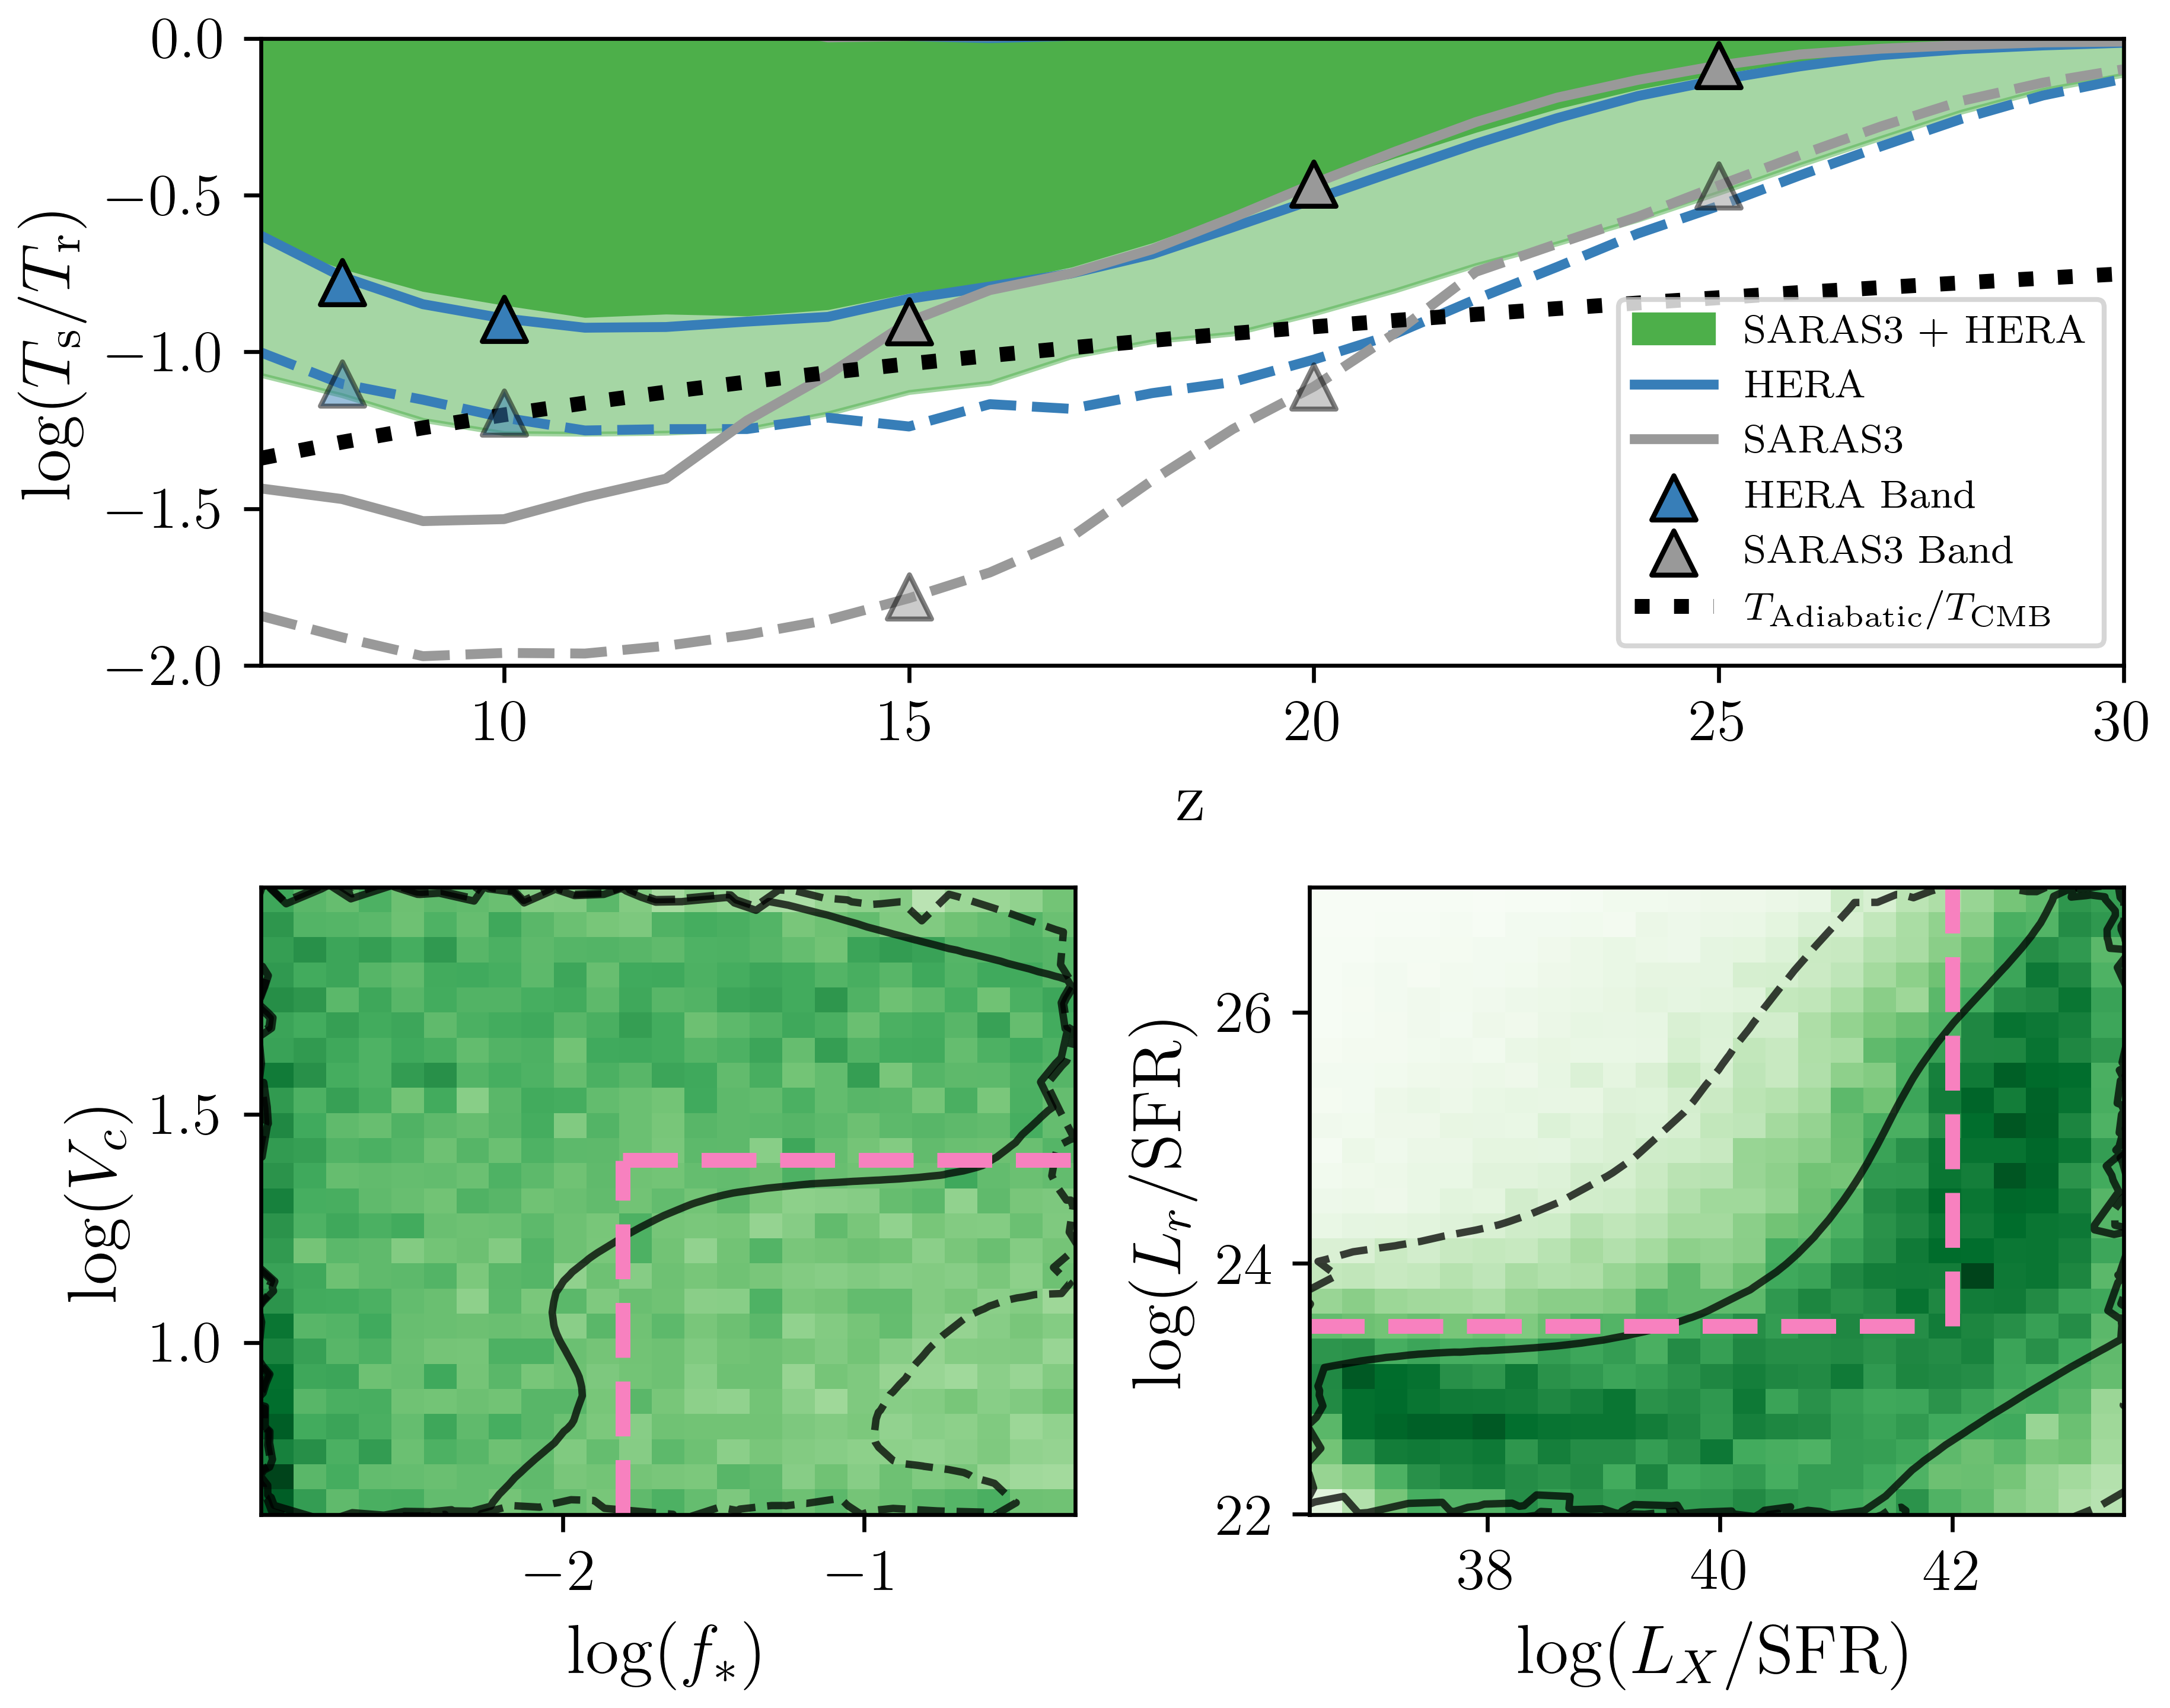
\includegraphics{joint_constraints/figs/TS_figure_4.png}
    \caption{\textbf{Key results from the joint analysis.} \textbf{Top Panel:} The ratio of the spin temperature of neutral hydrogen, $T_s$, and the radio background temperature, $T_r$, as a function of redshift for the joint HERA and SARAS3 analysis in green. We show the HERA and SARAS3 68\% and 95\% confidence constraints in blue and grey respectively as triangles at the relevant redshifts and solid and dashed lines. 
    As a guideline, we show the ratio for $T_r = T_{CMB}$ and assuming adiabatically cooled gas in an expanding Universe in the absence of any heating but with saturated coupling between $T_s$ and the gas kinetic temperature (dashed black line). 
    \textbf{Bottom Left:} The 2D probability distribution function~(PDF) from the joint analysis on the minimum virial circular velocity, $V_c$, in combination with the star formation efficiency, $f_*$, marginalising over $f_\mathrm{radio}$, $f_X$ and $\tau$. The solid black line shows the 68\% contour, approximated by the pink dashed line, and the black dashed line shows the 95\% contour. The joint analysis disfavours low values of $V_c$ and high $f_*$ corresponding to efficient star formation. \textbf{Bottom right:} The constraint on the X-ray and radio luminosities from the joint analysis marginalising over $V_c$, $f_*$ and $\tau$. The joint analysis disfavours at 68\% confidence low X-ray efficiencies in combination with high radio production efficiencies.}
    \label{fig:igm_params}
\end{figure}

Next, we explore the functional constraints in the $T_{21} - z$ and $\Delta_{21} - z$ planes as shown in \cref{fig:functional}. 
These are calculated by taking the samples of $\theta_{21}$ output from our fits and using the neural network emulators to produce corresponding global signals and power spectra. Using our theoretical models, we can easily map between the constraints on the power spectra and global signals. We see that for both the power spectra and the sky-averaged signals, although more clearly for the latter, the range of plausible models is reduced by our joint analysis. The signals that are inconsistent with the data typically have strong power spectra and corresponding deep absorption trough in the global signal, and belong to the models with weak X-ray heating and strong radio luminosity. Further, we see that the $2\sigma$ region for the functional constraints correspond to signals with the power spectra  $\lesssim 10^{2.1}$ mK$^2$ at $z=25$, which via our modelling maps to global 21-cm signals shallower than $-277$~mK. We note that the $3\sigma$ limit on the power spectrum at $z=25$ of $\lesssim10^{3.2}$ mK$^2$ is approximately equivalent to the expected sensitivity of NenuFAR from 1000 hours of observations \cite{Mertens_NenuFAR_2021}. For the global 21-cm signal, $3\sigma$ limit on the magnitude reduces from $\approx-2630$~mK from HERA to $\approx-1770$~mK from the joint analysis. Remarkably, we find that for the sky-averaged signal, the $2\sigma$ limit is very close to the minimum depth of the `standard astrophysical' models, $\approx -165$ mK \cite{Reis_sta_2021}, where the radio background is equated to the CMB, the contributions from radio galaxies and X-ray heating sources are assumed to be negligible, while the CMB and Lyman-$\alpha$ heating are present. The relatively tight constraints on the global signal and power spectrum suggest that future improved measurements  will allow us to dig deeper into the models with weak excess radio background radiation. It is clear from our analysis, that the joint constraint improves limits on the range of plausible global signals and power spectra.

\begin{figure}
    \centering
    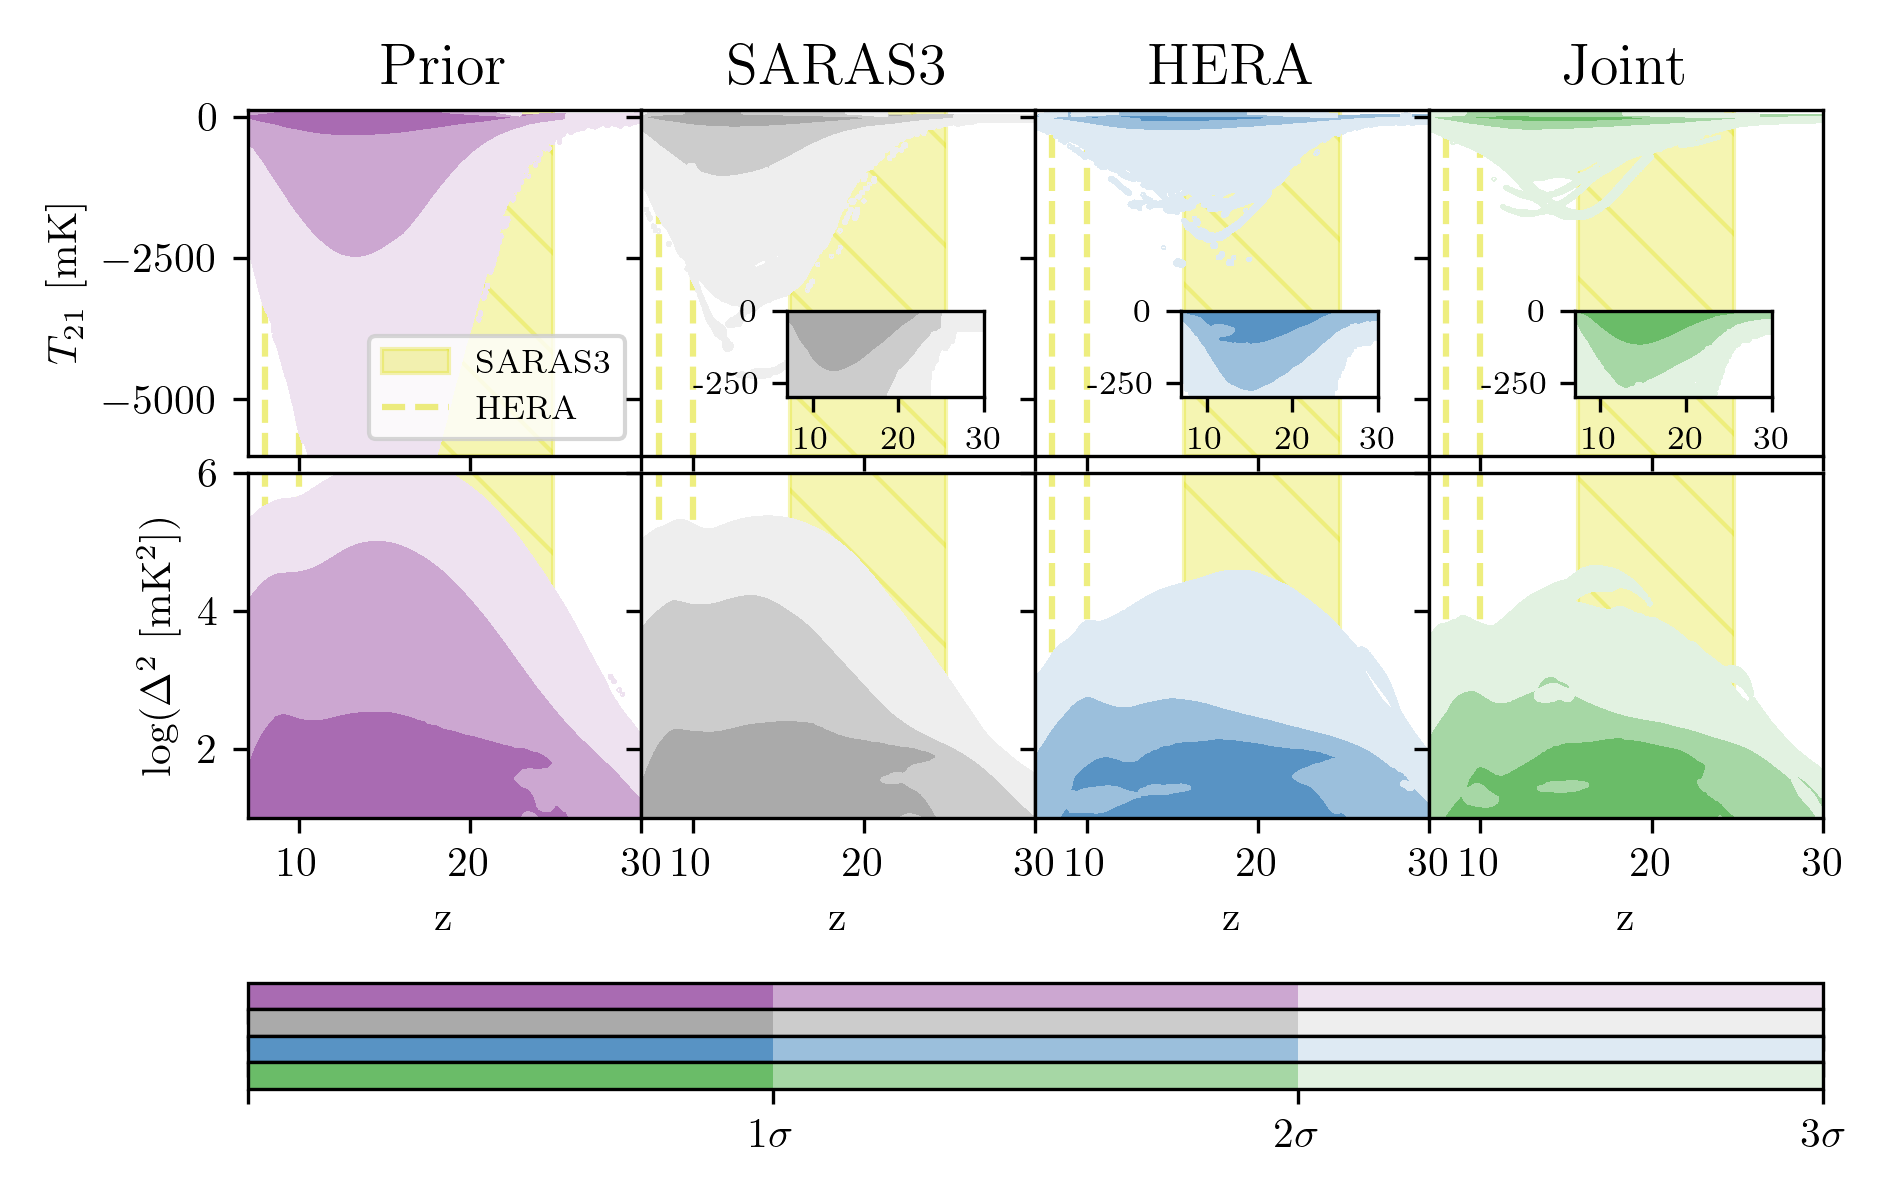
\includegraphics{joint_constraints/figs/fgivenx_plots.png}
    \caption{\textbf{Functional constraints on $T_{21}$ and $\Delta^2$.} The functional prior (purple), SARAS3 (grey), HERA (blue) and joint (green) posteriors for the sky-averaged 21-cm signal (top row) and power spectrum (bottom row). The yellow shaded region shows the SARAS3 band, and the dashed yellow lines show the HERA redshifts. The functional prior and posteriors are calculated by taking representative samples from the corresponding probability distributions for the astrophysical parameters and generating the corresponding signals using neural networks. We see that by combining the constraining power of HERA and SARAS3, we significantly reduce the $3\sigma$ (lightest shaded regions) constraints on the magnitude of both signals from $-2630$~mK to $-1770$~mK at $z=15$ for the global signal and $10^{3.7}$~mK$^{2}$ to $10^{3.2}$~mK$^{2}$ for the power spectrum at $z=25$. The figure is produced with \textsc{fgivenx} \cite{fgivenx}.}
    \label{fig:functional}
\end{figure}

We can now interpret the constraints on the temperatures in terms of the limits on the properties of the astrophysical sources modelled in the simulation. 
The key constraints from the joint analysis are shown in the  bottom panels of \cref{fig:igm_params} including the limits  on the high-redshift star formation which drives the high-redshift portion of the 21-cm signal via the process of Lyman-$\alpha$ coupling (constraints in the planes $V_c - f_*$) and the constraints on the luminosity of X-ray and radio sources ($L_r - L_X$) which primarily regulates the depth of the absorption trough. The full marginalised 1D and 2D posteriors corresponding to the joint analysis are shown in \cref{fig:posterior} and the key numerical results are summarized in \cref{tab:numbers_joint} where we list the individual constraints from SARAS3 and HERA along with the joint analysis. We find that the combination of the two experiments leads to stronger constraints in the two-dimensional probability distribution of $L_r - L_X$ than either of the two experiments individually. Where HERA constrains the population of high redshift radio-luminous galaxies to be $\lesssim400$ times brighter in the radio band than the current population, the combination of the data sets constrains the galaxies to be $\lesssim300$ times brighter when marginalising over the other parameters ($V_c$, $f_*$, $f_X$ and $\tau$). Similarly, HERA disfavours at 68\% confidence galaxies with an X-ray luminosity $\lesssim 0.25$ times the present day value in combination with the radio luminosity of galaxies in the early universe that is $\gtrsim 400$ times the present day value. The joint analysis provides a stronger constraint, ruling out scenarios where the X-ray luminosity is $\lesssim 33$ times the present day value and the radio luminosity of the first galaxies is $\gtrsim32$ times the present day value at 68\% confidence.

\def\arraystretch{1.5}
\begin{table}[]
    \centering
    \begin{tabular}{|p{2cm}|p{3.5cm}|p{3.5cm}|p{3.5cm}|}
         \hline
         & SARAS3 & HERA  & SARAS3 + HERA \\
         \hline
         \hline
         Signal & Sky-averaged & Power Spectrum & Both \\
         \hline
         $z$ & $\approx 15 - 25$ & $\approx 8$ \& $\approx 10$ & $\approx 8$, $\approx 10$ \& \newline $\approx 15 - 25$ \\
         \hline
         \hline
         $L_{r}/\mathrm{SFR}$ & $\gtrsim 1.55\times10^{25}$ & $\gtrsim4.00\times10^{24}$ & $\gtrsim3.31\times10^{24}$ \\
         \hline
         $L_{X}/\mathrm{SFR}$ & -- & $\lesssim7.60\times10^{39}$ & $\lesssim3.71\times10^{39}$ \\
         \hline
         $L_{r}/\mathrm{SFR}$ \& $L_{X}/\mathrm{SFR}$ & $\gtrsim 1.00\times10^{25}$ \& \newline $\lesssim 1.09\times10^{42}$ & $\gtrsim 4.00\times10^{24}$ \& \newline $\lesssim 7.60\times10^{39}$ & $\gtrsim 3.16\times10^{23}$ \& \newline $\lesssim 1.00\times10^{42}$ \\
         \hline
         $M$ & $4.40\times10^{5} \lesssim M \newline \lesssim 1.10\times10^{7}$ & -- & $2.55\times10^{5} \lesssim M \newline \lesssim 7.04\times10^{6}$\\
         \hline
         $f_*$ & $\gtrsim 0.05$ & -- & $\gtrsim 0.06$\\
         \hline
         $f_*$ \& $M$ & $\gtrsim 0.03$ \& \newline $\lesssim 8.53\times10^{8}$ & -- & $\gtrsim 0.02$ \& \newline $\lesssim 4.50\times10^{7}$\\
         \hline
    \end{tabular}
    \caption{\textbf{Key parameter constraints from SARAS3, HERA and the joint analysis.} Here the SARAS3 and HERA limits are taken from \cref{ch:saras3} and \cite{HERA_2022b}. In the top two rows, we show the type of signal targeted by each set of analysis and the corresponding redshifts. The joint analysis produces improved constraints on the radio and X-ray backgrounds, while retaining the constraining power of SARAS3 on the star formation properties of early galaxies. $L_r$ is measured in W~Hz$^{-1}$~M$_\odot^{-1}$~yr at a reference frequency of $150$~MHz, $L_X$ in erg~s$^{-1}$~M$_\odot^{-1}$~yr, and is calculated by integrating X-ray spectral distribution of sources between 0.2 and 95~keV  assuming an X-ray SED consistent with that for X-ray binaries \cite{Fragos_Xrays_2013}. The halo mass, $M$, is measured in solar masses. These constraints are derived from Kernel Density estimates~(KDE) of the 1D and 2D posterior distributions.}
    \label{tab:numbers_joint}
\end{table}

We find comparable constraints on $f_*$ and minimum mass of star forming halos, $M$, as was found with SARAS3 alone \citep[\cref{ch:saras3},][]{Bevins_saras3_2022} when combining the data sets, suggesting that HERA has no influence on our ability to determine high-redshfit star formation efficiencies or dark matter halo masses (or, equivalently, $V_c$). Marginalising over the radio and X-ray luminosities, we disfavour at 68\% confidence galaxies in which $\gtrsim2\%$ of the gas is converted into stars and the minimum mass for star forming halos is $\lesssim 45$ million solar masses.

Further, we explore the structure of the global 21-cm signals which are consistent with the data from SARAS3, HERA and the two sets together. We do this by looking at  the minimum  temperature, $T_\mathrm{min}$, the  corresponding central redshift, $z_0$, and an approximate full width at half max, $\Delta z$, of each absorption trough as defined in the top right of \cref{fig:tmin}. More specifically, for each parameter set $\theta_{21}$ (either from the prior parameter range, or from the posterior ranges consistent with SARAS3, HERA, and the joint analysis) we generate a global signal using the  neural network emulator \textsc{globalemu} \citep[\cref{ch:globalemu},][]{Bevins_globalemu_2021}. We then measure the values of $T_\mathrm{min}$, $z_0$, and  $\Delta z$ for each signal, producing probability distributions for each parameter corresponding to the constraints from each data and showing the extent of the prior (see results in \cref{fig:tmin}). We compare these distributions with the values used to parameterise the phenomenological EDGES flattened Gaussian signal with the EDGES 99\% confidence ranges shown by the black crosses in the corner plot in \cref{fig:tmin}. We see that when considered individually, the SARAS3 and HERA experiments allow for astrophysically motivated sky-averaged 21-cm signals that have a minimum temperature, location and width in agreement with the EDGES detection (i.e. the EDGES measurement overlaps with the 95\% contours), while the joint analysis rules out models with a depth that is consistent with EDGES at greater than a $2\sigma$ significance. The joint analysis has a preference for shallower (lower values of $|T_\mathrm{min}|$) and narrower signals with higher central frequencies, as can be seen in the corresponding 1D PDFs, which is driven largely by the HERA constraints.

\begin{figure}
    \centering
    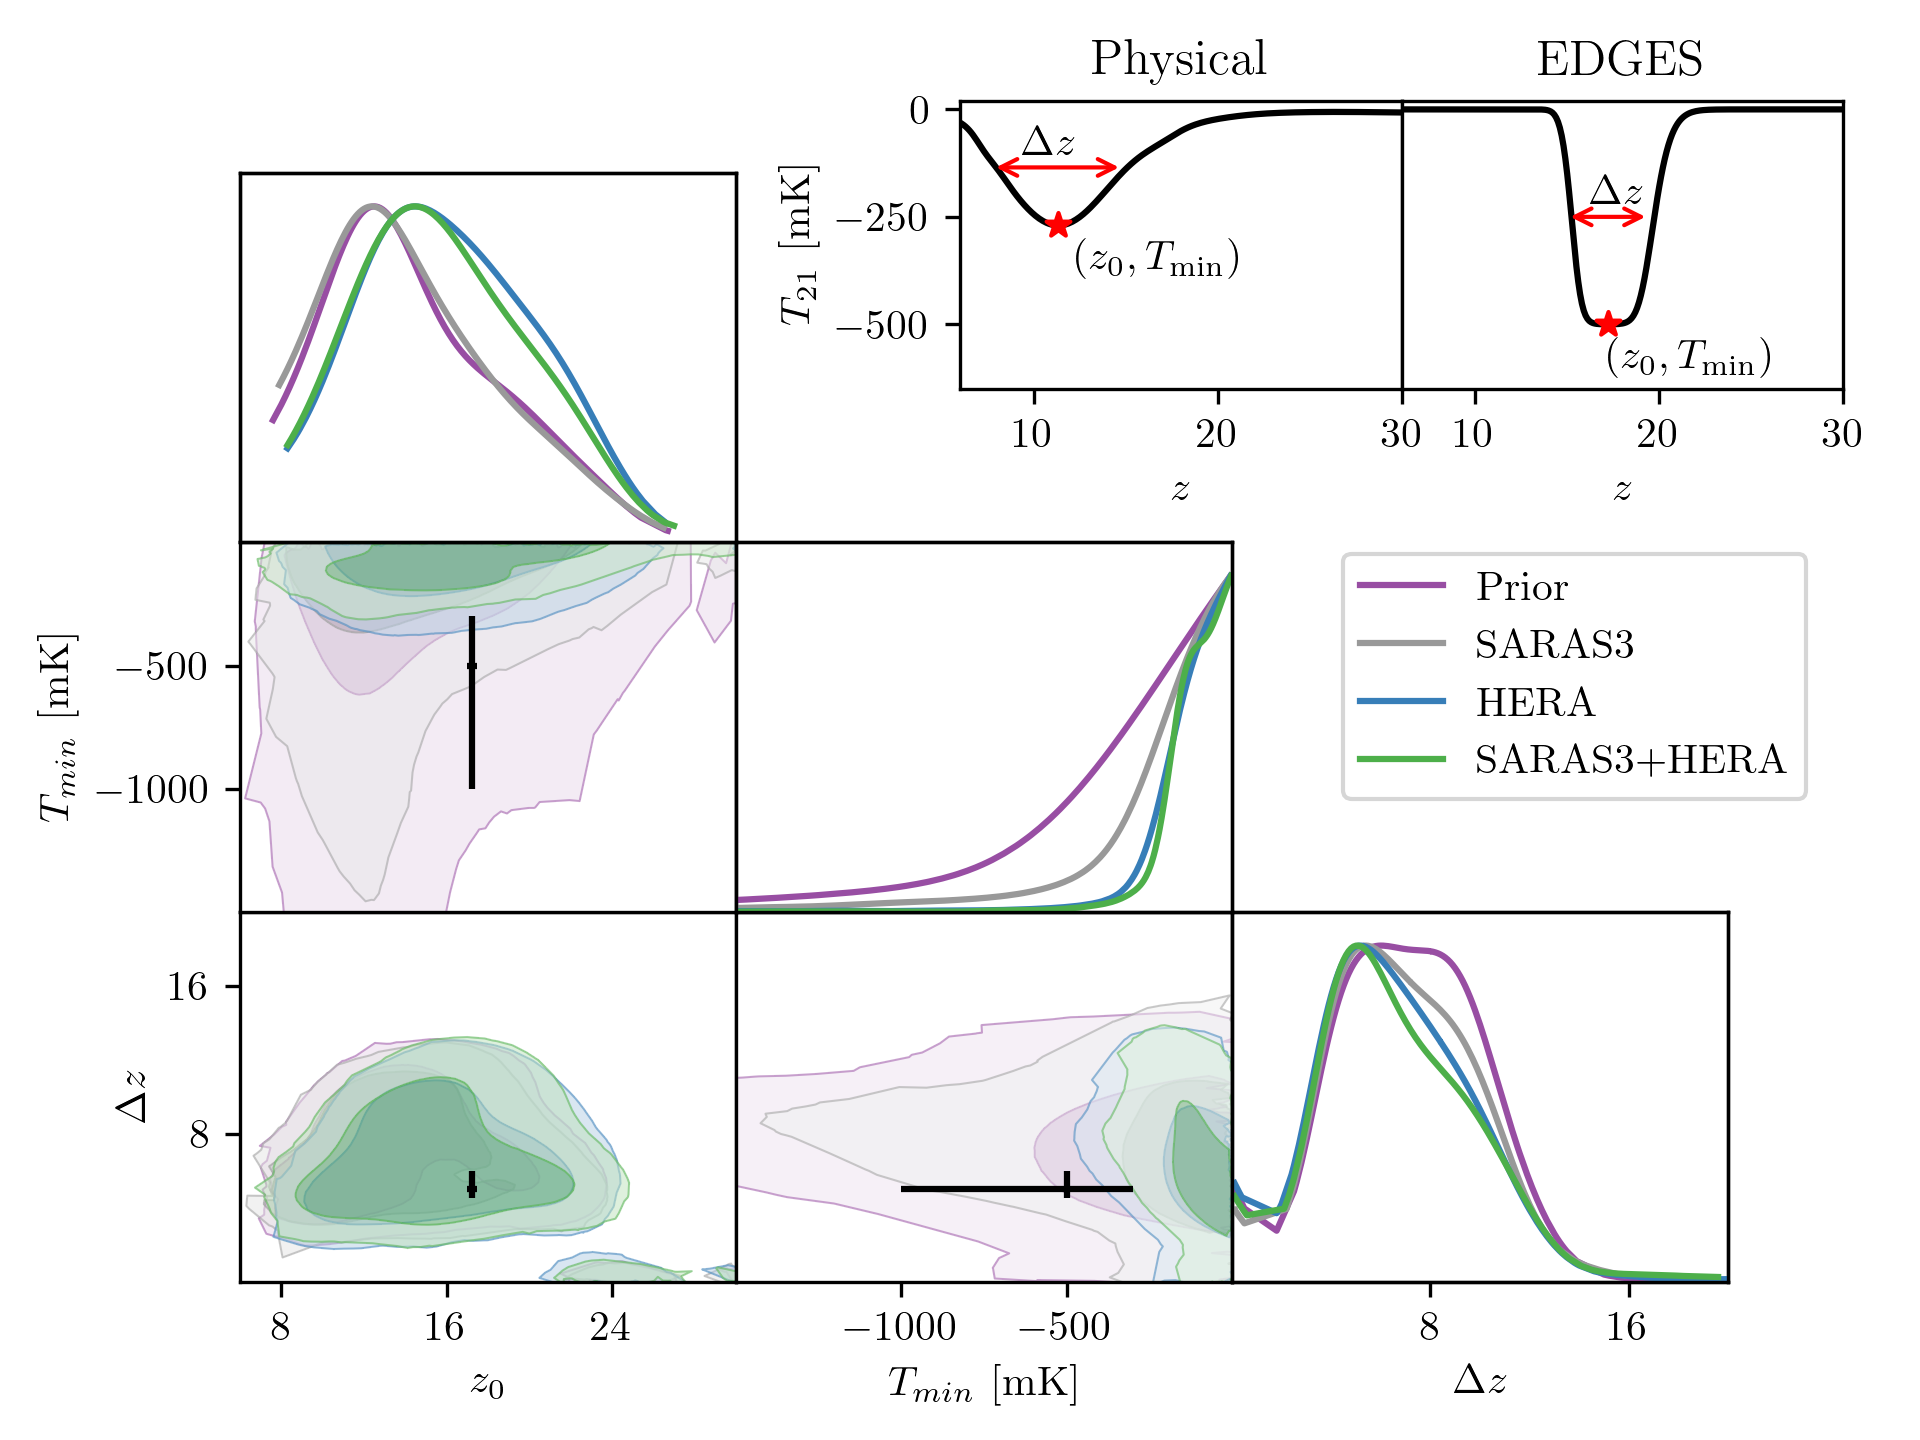
\includegraphics{joint_constraints/figs/amp_width_cz.png}
    \caption{\textbf{Phenomenological constraints.} The triangular plots shows the prior (purple) and posteriors (grey for SARAS3, blue for HERA, green for joint) of the features of a typical global absorption signal: the central redshift, $z_0$, the corresponding minimum temperature, $T_\mathrm{min}$, and the width of the signal, $\Delta z$, as is depicted in the top right corner. Darker shaded regions show $1\sigma$ constraints, lighter shaded regions show $2\sigma$ constraints. Overlaid on the posterior distributions are the 99\% confidence intervals, black crosses, reported for the corresponding phenomenological parameterisation of the EDGES absorption feature in \cite{Bowman_edges_2018}. Note that this is not the same as the physical EDGES-like distribution explored in \cref{fig:background}.
    We see that individually the experiments allow for  signals with depths that are consistent with EDGES. However, the combination of the two data sets disfavours these signals with greater than 2$\sigma$ significance. We do not disfavour signals with the same width or central frequency as EDGES, but note that the joint analysis indicates a preference for shallower and narrower signals with higher central redshifts as can be seen in the 1D PDFs.}
    \label{fig:tmin}
\end{figure}

We also consider the impact of SARAS2 on our joint constraints as well as that of MWA and LOFAR (with the latter two providing weaker constraints and thus having no effect), see \cref{sec:suplimentary_joint} for details.  We find that the addition of SARAS2 leads to an increased uncertainty in the star formation properties of galaxies in the infant Universe. This is likely because the SARAS2 data increases the envelope of plausible models at higher redshifts, where star formation dominates the structure of the 21-cm signal.
However, we note that even with its inclusion, we find a tight constraint on the combination of $L_r - L_X$. We focus in the main text on SARAS3 and HERA, due to the uncertainty in the modelling of and presence of systematic structures in the SARAS2 data, which is discussed in more detail in \cref{sec:suplimentary_joint}.

\section{Conclusion}\label{sec:conclusions_joint}

Through a combination of constraints on fluctuations and the sky-averaged 21-cm signal of neutral hydrogen, we have improved our understanding of the first galaxies that formed in the infant Universe between 200 and 700 million years after the Big Bang. This is the first time the data from the two different 21-cm probes have been combined to derive constraints on the astrophysical properties of the early galaxies. Even though the existing constraints are weak, we develop novel methodology and outline the approach which will become increasingly more useful as the  next-generation experiments  deliver stronger observational constraints. 

Considering a wide space of plausible astrophysical models including high-redshift sources of ultraviolet, X-ray and radio photons which affect the 21-cm signal, we calculate corresponding sky-averaged spectra as well as the power spectra of fluctuations. Using an upper limit on the fluctuations from the HERA interferometer and non-detection of the global 21-cm signal by the SARAS3 radiometer, we find that only $64.9^{+0.3}_{-0.1}$\% of the explored theoretical parameter space is consistent with the joint SARAS3 and HERA constraint, which is a significant improvement over the individual values of $92.3^{+0.3}_{-0.1}$\% and $79.0^{+0.5}_{-0.2}$\% respectively.

Using the newly developed methodology we place the tightest constraints to date on the properties of cosmic gas, such as the spin temperature of the 21-cm hydrogen line (closely related, but not equal, to the gas kinetic temperature) and the radio background temperature, $T_{r}$, as well as on the radio and X-ray luminosities of the first galaxies disfavouring at 68\% confidence galaxies that are approximately 32 times more efficient radio emitters than present galaxies and simultaneously are less than 33 times bright in the X-ray band. This work reports an increased degree of confidence over a wider range of redshifts than previous works which typically extrapolate outside the redshifts targeted by individual experiments, while here we interpolated between the observations of SARAS3 at $z = 15-25$ and the HERA limits at lower redshifts $z\sim8$ and 10. 

In this work, we also considered the addition of interferometric data sets from  MWA and LOFAR to our analysis, which led to a negligible improvement in the results. These experiments probe the physics of the EoR covering a similar redshift range to HERA (between $z\approx 6 - 10$), with the current HERA data providing the tightest constraints on our models. Of the current global or sky-averaged 21-cm experiments only SARAS2, SARAS3 and EDGES were able to place limits on the astrophysics of the infant Universe. Our main focus is on the SARAS3 limits, as there are concerns surrounding the cosmological nature of the signal reported in EDGES and a degree of uncertainty in the modelling of systematics in the SARAS2 data. We note that the SARAS2 data covers a similar redshift range as the HERA data and based on our analysis does not lead to a significant improvement in our constraints.

The new methodology developed in this chapter will allow for synergies to be explored between the upcoming observations, e.g. of the power spectrum from cosmic dawn measured by the NenuFAR \cite{Zarka_nenuFar_2018}, HERA, LOFAR or the SKA \cite{Mellema_SKA_2013}, as well as the measurements of the global signal by the wide-band REACH experiment covering the redshift range $z\approx 7 - 28$ \cite{de_lera_acedo_reach_2022},  PRIZM \cite{Philip_PRIZM_2019}, MIST \cite{MIST} and missions to the moon \cite{Burns_Moon_2021} among others. 

\renewcommand\thefigure{\arabic{chapter}.S.\arabic{figure}}
\renewcommand\thetable{\arabic{chapter}.S.\arabic{table}}
\renewcommand\thesubsection{\arabic{chapter}.S.\arabic{subsection}}
\renewcommand\thesection{\arabic{chapter}.S}
%\section{Supplementary Material} \label{sec:method_joint}

\setcounter{figure}{0}
\setcounter{table}{0}

\section{Supplementary materials} \label{sec:suplimentary_joint}

\subsection{Modelling the Thermal History of the Infant Universe: Power Spectrum and Global Signal Synergies}
\label{sec:modelling_joint}

At high redshifts around $z\approx 20 - 30$, the first stars begin to form and produce Lyman-$\alpha$ photons that interacts with the baryonic matter, predominantly composed of neutral hydrogen, in the Universe. Neutral hydrogen atoms absorb and remit ambient Lyman-$\alpha$ photons in a process known as the Wouthuysen-Field~(WF) effect \cite{Wouthuysen1952, Field1959} that drives the relative number of atoms with aligned and anti-aligned proton and electron spins. This process couples the spin temperature of the neutral hydrogen, $T_s$, which describes the distribution of hydrogen atom spins, to the gas temperature, $T_k$, which is cooling at a faster rate than the radio background as the Universe expands. Further, interactions between the neutral hydrogen and Lyman-$\alpha$ emission result in the transfer of kinetic energy that raises the gas temperature, and coupled spin temperature, in a process known as Lyman-$\alpha$ heating \cite{Madau1997, Chuzhoy2007} preventing the gas from cooling adiabatically. However, despite the heating, the dominant WF effect produces an absorption feature in the sky-averaged 21-cm signal, which is measured relative to the radio background. Further, it leads to a peak in the power spectrum at high $z \approx 25$ on angular scales corresponding to the effective horizon of the Lyman-$\alpha$ emission and the distribution of galaxies, which disappears when the coupling becomes saturated \cite{Cohen_power_2018}. The intensity and spatial fluctuations of the Lyman-$\alpha$ emission evolve with the population of early galaxies, and consequently it is dependent on their star formation rate and the minimum halo mass for star formation. We parameterize these quantities with the star formation efficiency, $f_*$, which quantifies the percentage of the baryonic mass in the star forming halos that is converted into stars, and the minimum virial circular velocity, $V_c$,  which is proportional to the cube root of the halo mass, $M$.

At intermediate redshifts of $z\approx 10 -20$ the gas is further heated by X-ray binaries \cite{Fragos_Xrays_2013, fialkov_observable_2014}, continuing Lyman-$\alpha$ heating, CMB heating \cite{Venumadhav2018} and heating through structure formation. X-ray heating is dependent on processes such as X-ray production in high redshift galaxies and black hole binary formation. This means that it has to be separately parameterized and in our semi-numerical simulations, we model the X-ray production efficiency, $f_X$, which is directly proportional to the X-ray luminosity per star formation rate, $L_X/$SFR measured in erg~s$^{-1}$~M$_\odot^{-1}$~yr, between 0.2 and 95~keV. The heating affects the redshift of the minimum and depth of the sky-averaged 21-cm signal. If sufficiently efficient it can raise the temperature of the gas, and coupled 21-cm brightness temperature, above the radio background resulting in emission in the sky-averaged signal at low redshifts. The heating rate has a direct impact on how fast the brightness temperature transforms from absorption to 0~K or emission. In the power spectrum, due to the non-uniformity of the heating, the various mechanisms can produce a peak in the signal at around $z\approx 15$. Although this redshift is model dependent (see \cite{Cohen_power_2018}) and in some cases when heating is done by hard X-rays (energies $>1$ keV with long mean free paths) X-ray heating is smooth and no peak is imprinted in the power spectrum \cite{fialkov_observable_2014, Fialkov_rich_2014}.

Finally, at more recent times, $z \approx 5 - 15$, ultraviolet emission from the first massive galaxies begins to ionize the neutral hydrogen, stripping the abundant gas of its electrons. This reduces the sky-averaged 21-cm signal and when reionization is complete, the signal disappears. The process produces a peak in the power spectrum at the scales corresponding to the typical size of ionized bubbles, but again the signal is destroyed once reionization is complete. The process of reionization is highly dependent on the ionizing efficiency of sources, $\zeta$, which in the models explored here is normalized by the CMB optical depth, $\tau$. While $\tau$ has been weakly constrained by cosmological experiments such as Planck \cite{Planck2018}, we treat it as a free parameter and note that 21-cm cosmology offers a means by which to break degeneracies between $\tau$ and other cosmological parameters.

\subsection{Combining Constraints with \textsc{margarine}}

We use the marginal Bayesian statistics code \textsc{margarine} \cite{margarine_neurips} to combine constraints from different data sets. \textsc{margarine} is outlined in \cref{ch:margarine} but to recap it uses neural networks known as Masked Autoregressive Flows (MAFs) to model the probability distribution, $\mathcal{P}(\theta|D, \mathcal{M})$, of a set of samples, here~{$\theta_{21}$}, marginalising over nuisance parameters describing the instrumental systematics, $\theta_{I}$, and foregrounds, $\theta_{fg}$ in the process. It does this by shifting and scaling a base standard normal distribution, making the probability of the distribution easily tractable, to replicate the target samples, where the shifting and scaling are determined by the outputs of the MAFs. 

This can subsequently be used to calculate a nuisance-free likelihood given a prior distribution and the Bayesian evidence using
\begin{equation}
    \mathcal{L}(\theta_{21}) 
\equiv \frac{\int\mathcal{L}(\theta_{21},\alpha)\pi(\theta_{21},\alpha)d\alpha}{\int \pi(\theta_{21},\alpha)d\alpha} = \frac{\mathcal{P}(\theta_{21}|D, \mathcal{M})\mathcal{Z}}{\pi(\theta_{21})},
    \label{eq:partial_joint}
\end{equation}
where $\alpha = \{\theta_{I}, \theta_{fg}\}$ \cite{margarine_maxent}. In instances when the prior is flat, then the following is true up to a normalisation constant
\begin{equation}
    \mathcal{L}(\theta_{21}) \approx \mathcal{P}(\theta_{21}|D, \mathcal{M}).
\end{equation}

With \textsc{margarine} we can subsequently evaluate $\log \mathcal{L}(\theta_{21})$ for any set of $\theta_{21}$ for any existing posterior distribution, $\mathcal{P}(\theta|D, \mathcal{M})$, from previous analysis of a data set like HERA or SARAS3
\begin{equation}
    \theta = \{\theta_{I}, \theta_{fg}, \theta_{21}\} \rightarrow \{\theta_{21}\} \rightarrow \textsc{margarine} \rightarrow \log \mathcal{P}(\theta_{21}|D, \mathcal{M}) \rightarrow \log \mathcal{L}(\theta_{21}),
\end{equation}
where the $\log$ is base 10. The likelihood evaluations can then be combined,
\begin{equation}
    \log \mathcal{L}_{\textnormal{joint}}(\theta_{21}) = \log \mathcal{L}_{\textnormal{HERA}}(\theta_{21}) + \log \mathcal{L}_{\textnormal{SARAS3}}(\theta_{21}),
\end{equation}
as discussed in the main text, to be sampled over using MCMC methods or in our case Nested Sampling implemented with \textsc{polychord} \cite{Handley2015a, Handley2015b}. 

%MCMC sampling methods approximate the unnormalised posterior distribution by directly sampling the product $\mathcal{P}(\theta) \approx \mathcal{L}(\theta)\pi(\theta)$ and do not provide estimates of the evidence, $\mathcal{Z}$. The family of algorithms typically use random walkers to traverse the parameter space, with points accepted and rejected based on some probabilistic criteria in an effort to explore the space fully. The HERA analysis \cite{HERA_2022b} of the excess radio background models explored here used the \textsc{emcee} \cite{Foreman_Mackey_2013} implementation of MCMC sampling \cite{HERA_2022b}.

%Nested sampling \cite{skilling_nested_2004} numerically approximates the integral
%\begin{equation}
%    \mathcal{Z} = \int \mathcal{L}(\theta)\pi(\theta) \delta \theta,
%\end{equation}
%which can be derived from \cref{eq:bayes} and the requirement that the posterior must integrate to 1, by evolving a series of live points to higher and higher likelihood values. By approximating the evidence, the algorithm produces samples on the normalised posterior distribution, which we subsequently use to determine preferred and disfavoured regions of the parameter space. A comprehensive review of Nested Sampling can be found in \cite{Ashton_ns_review_2022}.

\subsection{Emulating Signals from the EoR and CD}

%As described in the main text, semi-numerical simulations typically have a runtime of multiple hours for a given set of astrophysical parameters, thus performing parameter inference with the simulation directly is very costly. However, as both the sky-averaged signal and the power spectrum change smoothly when we vary parameters, we can interpolate values at intermediate parameters from existing simulations. An increasingly common practice to achieve this are the fast and precise neural network based emulators we discuss in the following sections.

\subsubsection{The sky-averaged 21-cm signal}

To emulate the sky-averaged 21-cm signal in models with an excess radio background from high redshift radio-luminous galaxies, we use the publicly available emulator \textsc{globalemu} described in \cref{ch:globalemu} and \cite{Bevins_globalemu_2021} trained on sets of astrophysical simulations. The simulations include the effects of Lyman-$\alpha$ and CMB heating. The mean free path of ionizing photons, $R_\mathrm{mfp}$, is fixed at $40$~Mpc and X-ray heating is powered by a population of X-ray binaries with a realistic spectral energy distribution \cite{fialkov_observable_2014}. The models correspond to the parameterisation detailed above and in \cite{Reis2020}.

The emulator has previously been used in the individual analysis of data from SARAS2 \cite{Bevins_SARAS2_2022} and SARAS3 \cite{Bevins_saras3_2022} and detailed in the corresponding papers and chapters. We therefore only briefly summarise the accuracy of the neural network here. The original set of simulations comprise approximately 10,000 models however the explored range of $\tau$, the CMB optical depth, is large and when training our neural network we filter out models that have a value of $\tau$ outside the range given by Planck $\pm 3\sigma$. This results in a training set of approximately 4,300 models, and the network is tested on approximately 500 models. A root mean squared error~(RMSE) of 5.11~mK is found and a 95 percentile RMSE of 20.53~mK indicating a high level of accuracy~(see \cref{ch:saras3}).

\subsubsection{The 21-cm power spectrum}
\label{sec:power_spec_emulation}

For comparing models with the HERA measurements we use the same 21-cm power spectrum emulator used in the HERA analysis \cite{HERA_2022b}, based on the same suit of simulations of the sky-averaged signal emulator used in the SARAS2 and SARAS3 analysis.
Based on an input of the 5 model parameters, this emulator returns the 21-cm power spectrum with a relative accuracy of 20\% at the wave numbers and redshifts observed by HERA. 
For HERA the impact of $\tau$ is more significant because the data corresponds to lower redshifts and so the full prior range on the parameter is used for training. This results in a training set of $\sim$8,000 simulations and another 2,000 independent samples for testing. Full details and tests of this emulator can be found in the HERA analysis paper \cite{HERA_2022b}, Appendix B.

We note that when performing our joint analysis we use the narrow prior on $\tau$ defined by Planck, since the SARAS3 posterior is not defined in the original analysis for values outside this range.

\subsubsection{Temperatures}
\label{sec:igm_temperature_emulation}

To emulate physical properties such as the spin temperature and temperature of the radio background (as seen in Figure \ref{fig:igm_params}) we use a \textsc{globalemu}-style emulator. In this framework, the emulator takes in the five astrophysical parameters and a single redshift and returns a single corresponding temperature. In practice, this means that vectorised calls have to be made to emulate the spin temperature, $T_s(z)$, and the radio background temperature, $T_r(z)$, as a function of redshift, but the method is found to be more accurate, quicker and allows for interpolation at a range of different redshifts. We use the same training and test sets as used for the 21-cm power spectrum emulator, and a similar architecture of 4 layers, with a reduced size of 100, 30, 10, and 5 nodes per layer. This allows us to emulate the spin temperature $T_s$ within $\pm 6\%$ accuracy (95\% confidence interval), and the radio background temperature $T_{r}$ within $\pm 4\%$ accuracy (95\% confidence interval). These neural networks and the power spectrum network were developed by Stefan Heimersheim.

\subsection{Constraints on the Astrophysical Parameters}

\Cref{fig:posterior} shows the 1D and 2D marginal posteriors found for the joint analysis of SARAS3 and HERA. The graph shows that the combined constraining power of the two experiments leads to a strong constraint on the combination of the radio and X-ray luminosities per star formation rate for an early population of galaxies when marginalising over the other astrophysical parameters. We also see constraints in the plane of $V_c - f_*$ when marginalizing over the radio background and X-ray heating parameters. The constraints are summarized in detail in the main text.

\begin{figure}
    \centering
    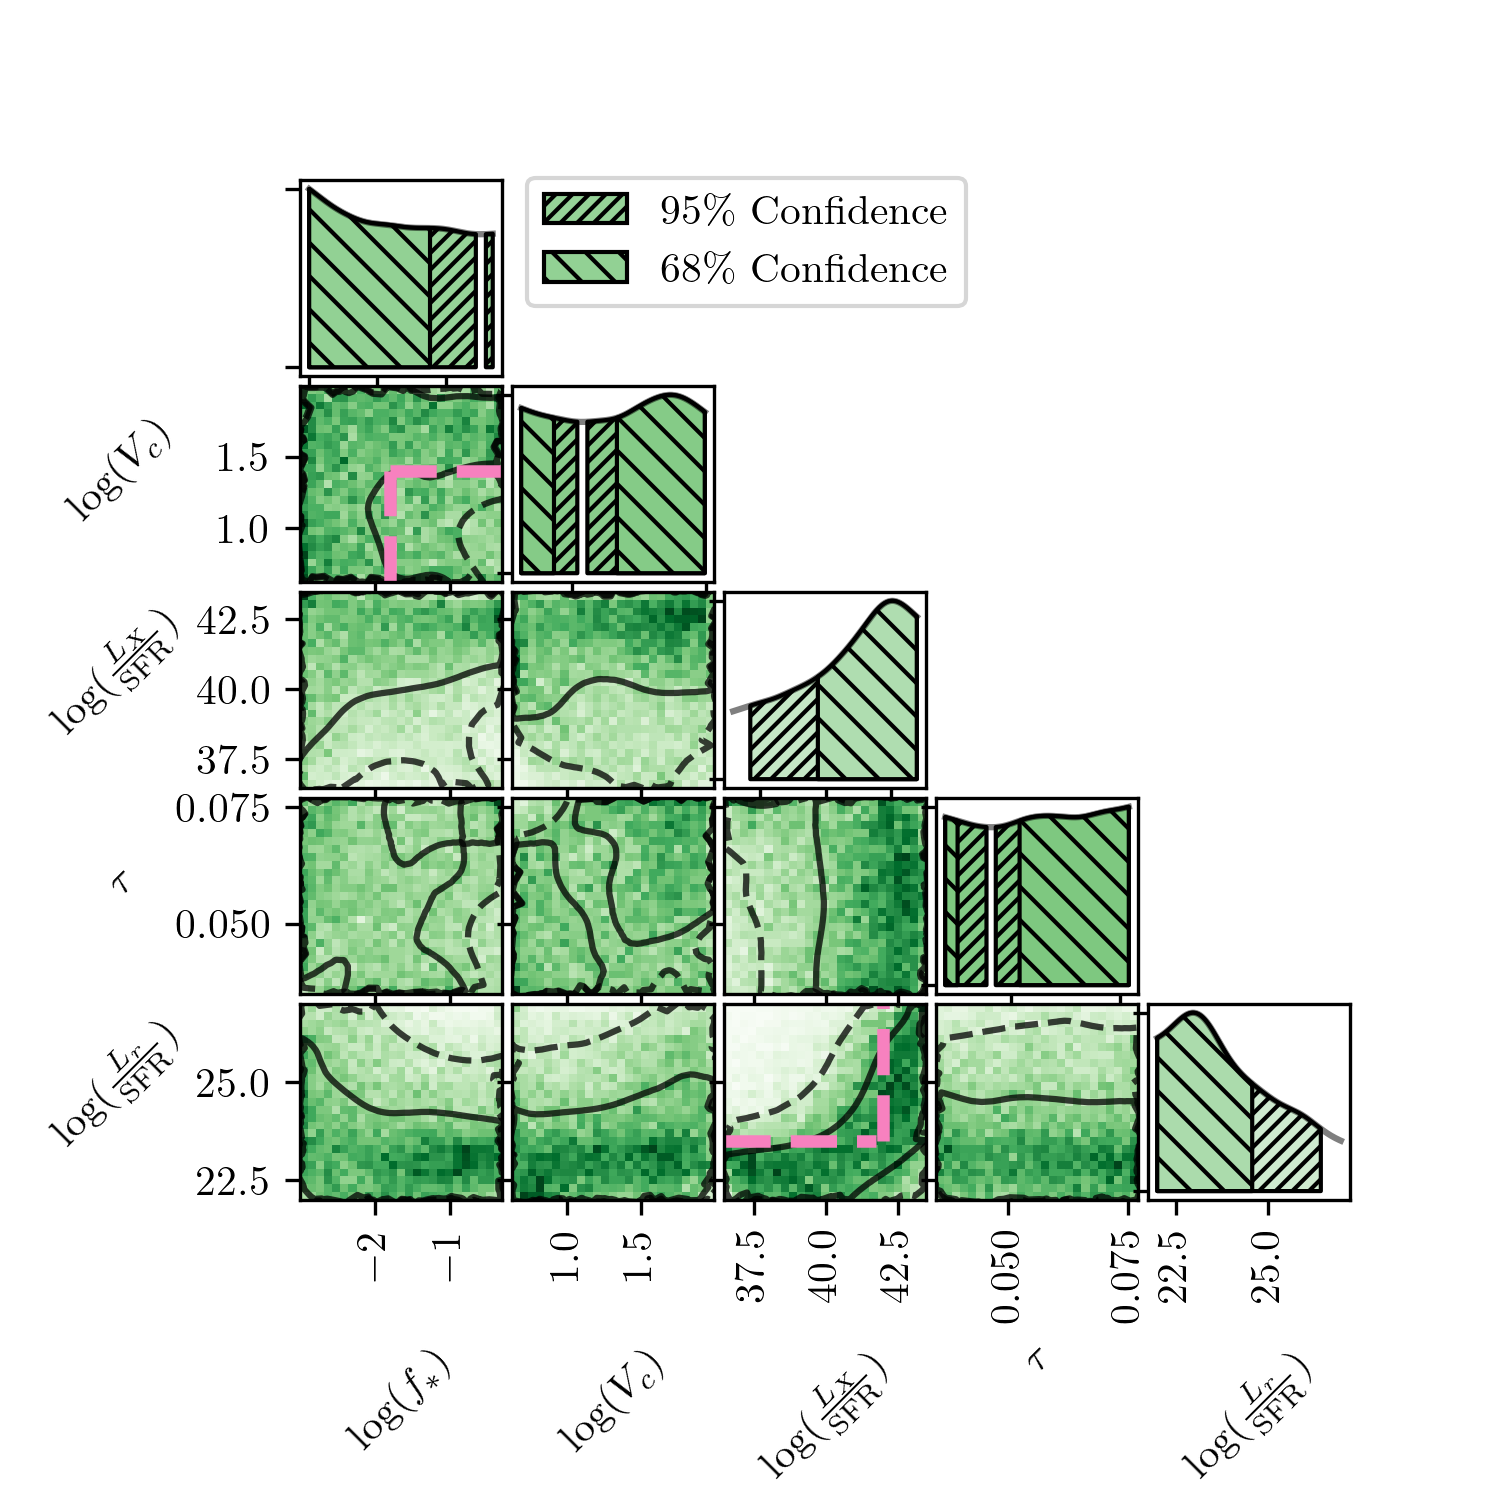
\includegraphics{joint_constraints/figs/hera_saras3.png}
    \caption{\textbf{Parameter constraints from the joint anlaysis.} The astrophysical parameter constraints on models with excess radio background in addition to the CMB derived when combining an upper limit on the 21-cm power spectrum at $z\approx8$ and $\approx 10$ from HERA with data from the 21-cm sky-averaged experiment SARAS3 in the band $z\approx15-25$. Through the combination of these two data sets probing different statistical properties of the 21-cm signal at different redshifts, we are able to improve constraints on the radio and X-ray luminosities of early radio-luminous galaxies and maintain constraints provided by SARAS3 on the star formation properties of these early galaxies. $L_r$ is measured in units of W~Hz$^{-1}$~M$_\odot^{-1}$~yr at 150~MHz and $L_X$ is in units of erg~s$^{-1}$~M$_\odot^{-1}$~yr calculated between 0.2 and 95~keV assuming a realistic SED of an early X-ray binary population. The pink dashed lines approximate regions that are disfavoured with 68\% confidence.}
    \label{fig:posterior}
\end{figure}

\subsection{Constraints on the Radio and X-ray Backgrounds}

\begin{figure}
    \centering
    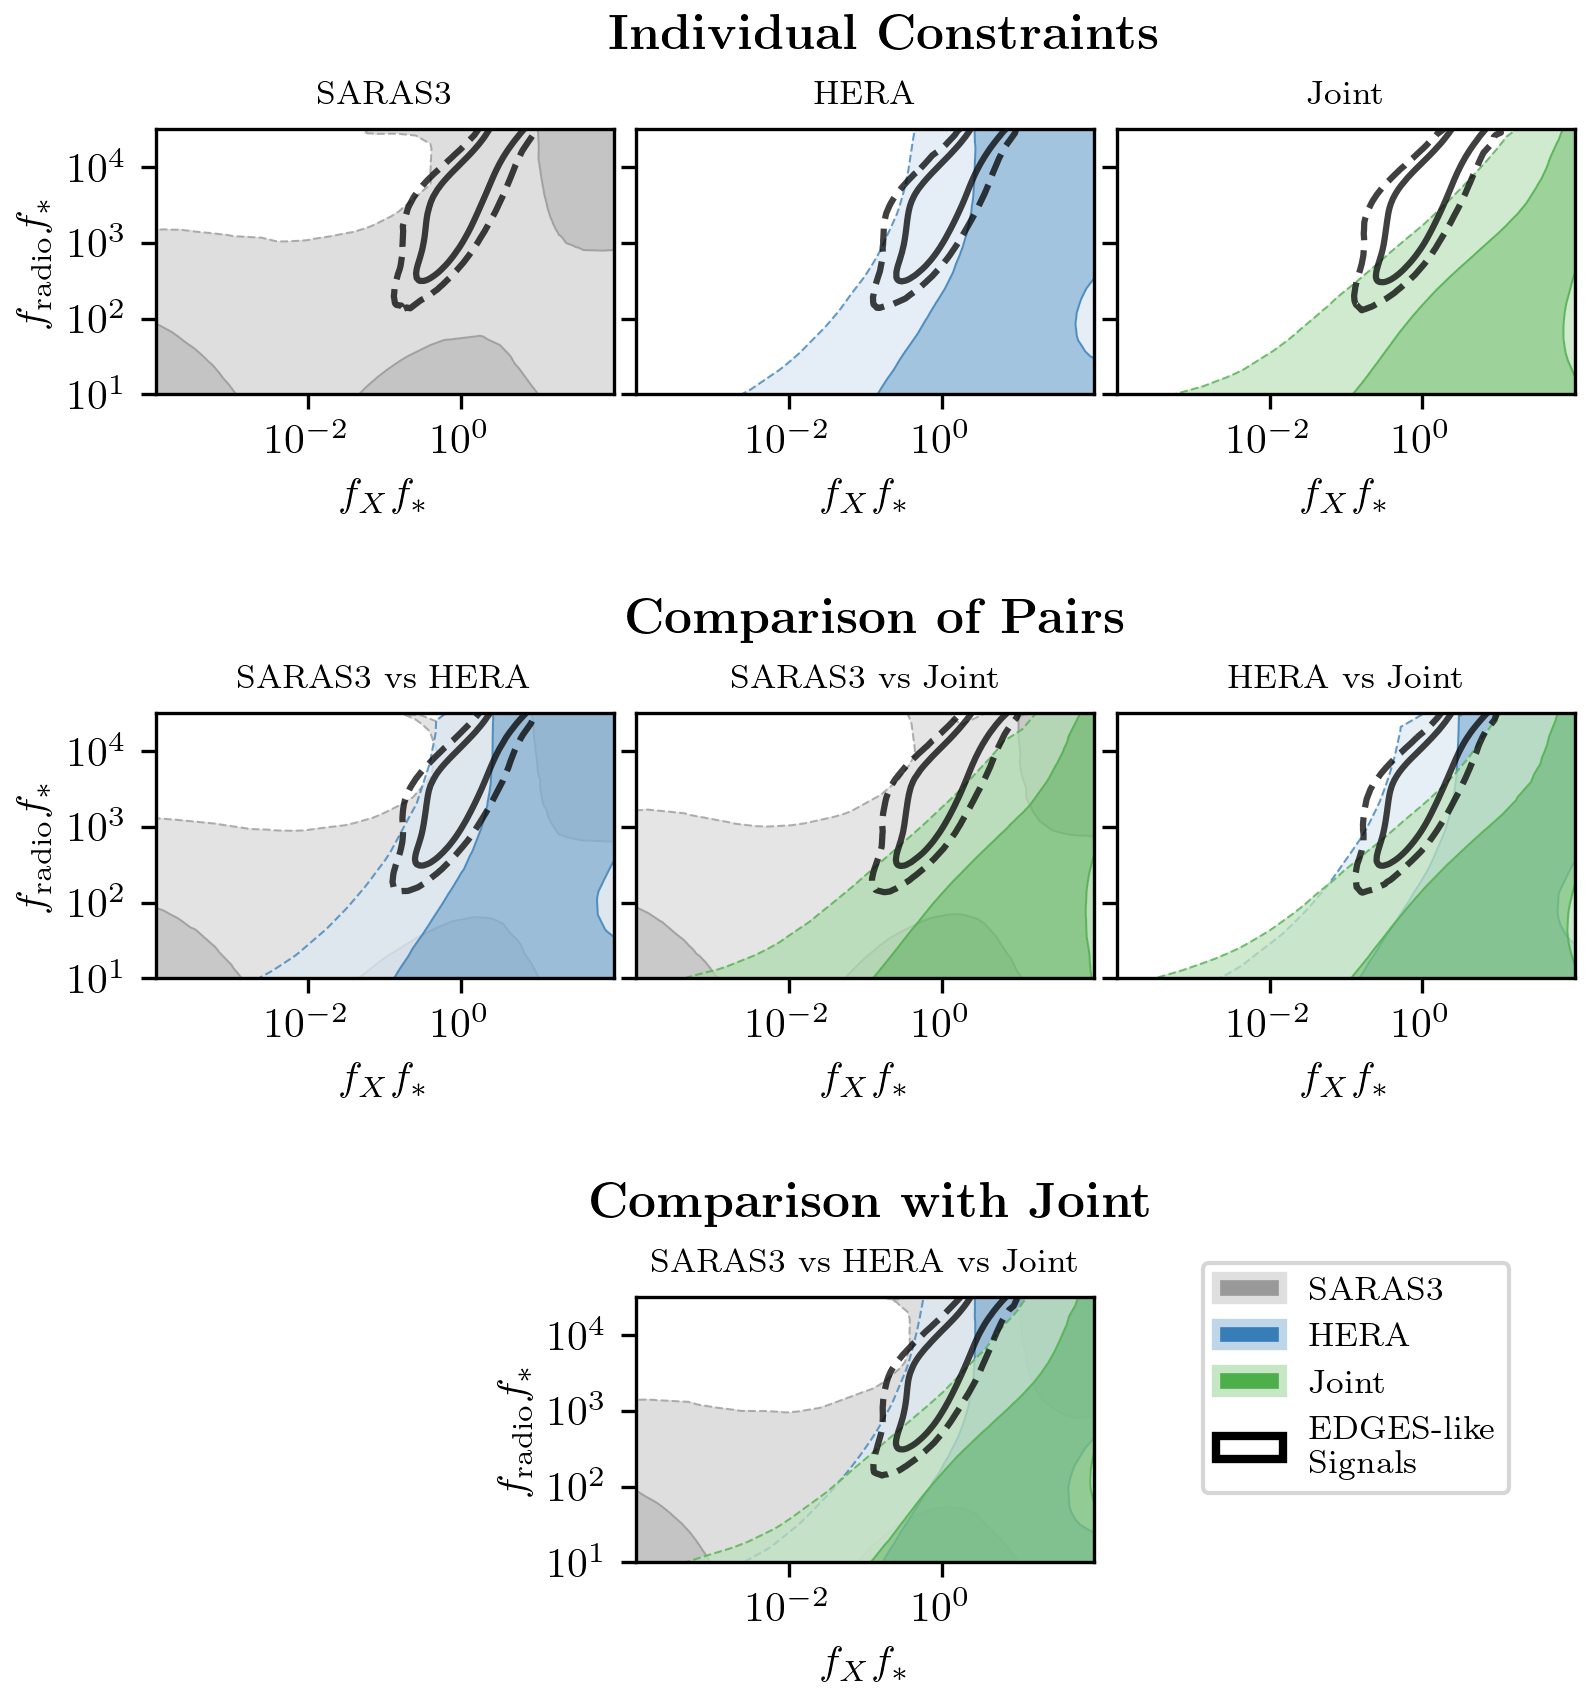
\includegraphics{joint_constraints/figs/xray_vs_radio_background_test.png}
    \caption{\textbf{Background constraints.} The figure shows constraints on the radio and X-ray backgrounds, parameterized by $f_* f_\mathrm{radio}$ and $f_* f_X$ respectively, from SARAS3 (grey), HERA (blue) and the joint analysis (green). The SARAS3 and HERA posteriors are based on the results presented in \cite{Bevins_saras3_2022} and \cite{HERA_2022b} respectively. We show each distribution individually on the top row, overlaid pairs of distributions for comparison in the middle, and all three on the same figure in the bottom row. In all panels, we show 68\% and 95\% contours (black solid and dashed lines respectively) for physical signal models that have similar depths and central frequencies as the EDGES absorption feature as defined by the inequality in \cite{Fialkov2019}. These physical EDGES-like models have previously been explored in the literature in \cite{Fialkov2019, Reis2020}. We note that while individually both HERA and SARAS3 allow for astrophysically motivated signal models that could explain the depth of the EDGES feature, together they rule the corresponding parameter space out with approximately greater than $2\sigma$ confidence, although some EDGES-like signals are still viable. We stress, again, that the explored physical models cannot fully explain the shape of the EDGES signal.}
    \label{fig:background}
\end{figure}


The product  $f_* f_\mathrm{radio}$ is proportional to the total radio background created by radio-luminous galaxies, and, equivalently, $f_* f_X$ is a proxy for
the total X-ray background created by the early population of X-ray sources. This is demonstrably true for our model parameterisation as the star formation rate is proportional to $f_*$ and the radio luminosity and X-ray luminosities per star formation rate are proportional to $f_\mathrm{radio}$ and $f_X$ respectively. Both X-ray and radio backgrounds are responsible for regulating the depth of the absorption feature, and they can also be observed independently by other telescopes (e.g. observations of the unresolved X-ray background by Chandra \cite{Lehmer_Chandra_2012} and of the low-frequency radio background by ARCADE2/LWA \cite{fixsen_arcade_2011, dowell_radio_2018}). In \cref{fig:background} we show constraints on the values of $f_*~f_X$ and $f_*~f_\mathrm{radio}$ achieved by SARAS3, HERA and the joint analysis. Since these combinations of the parameters regulate the absorption depth of the global 21-cm signal, we can also condition our prior on the astrophysical parameters to produce signals with the same central frequency and depth as the absorption feature found in the EDGES data \cite{Fialkov2019, Reis_sta_2021, Bevins_saras3_2022}. In each panel of \cref{fig:background}, we show black contours corresponding to these EDGES-like physical signals. We see that while HERA and SARAS3 allow for combinations of $f_X~f_*$ and $f_\mathrm{radio}~f_*$ that could  partially explain EDGES, the combination of the two experiments, which produces a tighter constraint on the X-ray and radio luminosities of early galaxies, disfavours a large portion of the EDGES-like parameter space (i.e. most of the EDGES-like parameter space is beyond the 95\% contours of the joint constraints, while it is well within the 95\% contours for SARAS3 and HERA individually). This demonstrates further the power of combining different data sets. However, we note that the explored theoretical signals do not fit EDGES data well, as none of the models closely reproduce the flattened Gaussian-like feature found in the data \cite{Bowman_edges_2018}.

\subsection{The impact of SARAS2}

Previous analysis of the SARAS2 data revealed some weak constraints, most notably in the plane of $L_X - L_{r}$ in agreement with HERA and SARAS3, on the properties of galaxies in the infant Universe \citep[e.g \cref{ch:saras2},][]{Bevins_SARAS2_2022}. SARAS2 is at much lower redshifts than SARAS3 but overlaps with the redshifts probed by HERA having recorded observations in the band $z\approx7-12$. The data is contaminated by a sinusoidal systematic and a number of different models were fitted to this feature. The models correspond to a signal introduced prior to the antenna possibly from ground emission or some unknown component of the foreground, and separately a signal introduced in the system electronics potentially from cable reflections. The sinusoidal systematic was fitted alongside a signal model generated with \textsc{globalemu} and a foreground model that is conditioned to be smooth preventing it fitting out non-smooth systematics or signals in the data \cite{Bevins_maxsmooth_2021}. Here we take the best fitting model, with a systematic from ground emission or a non-smooth component from the foreground, with the highest evidence from the original analysis \citep[see \cref{ch:saras2} and ][]{Bevins_SARAS2_2022} and combine the corresponding constraints on the astrophysical parameters $V_c$, $f_*$, $f_X$, $f_\mathrm{radio}$ and $\tau$ with the joint constraints from HERA and SARAS3 to assess the impact.

As can be seen in \cref{fig:other_global}, the addition of SARAS2 to our analysis washes out the constraint in the plane $f_* - V_c$. One possible explanation for this is that the addition of SARAS2, while constraining the properties that affect the signal at low redshifts, increases the envelope of possible models at higher redshifts, where star formation is more important, that are plausible even given the constraints from the SARAS3 data. Despite this, we note that we maintain the constraint in the plane $L_X - L_r$ when we add SARAS2 into our analysis.

We can quantify the impact of SARAS2 on our analysis by looking at the percentage of the astrophysical prior volume which is consistent with the different combinations of the three different data sets. To calculate this percentage, we use \textsc{margarine} to calculate the marginal Kullback-Liebler divergence, $\mathcal{D}$, between the flat prior on the five astrophysical parameters in the set $\theta_{21}$ and the corresponding posteriors. The KL divergence is related to the percentage via
\begin{equation}
    \% = 100\times\exp(-\mathcal{D}) \approx 100 \times \frac{V_\mathcal{P}}{V_\pi},
\end{equation}
where $V_\pi$ is the prior volume and $V_\mathcal{P}$ is the posterior volume. This quantity is useful as it quantifies the constraining power of the different data sets in all five dimensions, including correlations that may not be visible in the one and two-dimensional projections used to produce the corner plots in this chapter and in the literature. 

We show in \cref{fig:volume_contraction} the percentage of the astrophysical parameter prior volume that is consistent with different combinations of the data sets discussed in this work~(including additional interferometric measurements of the power spectrum discussed in \cref{sec:other_interferometers}). We see that the combination of either or both of the SARAS data sets with HERA lead to a percentage consistency with the data of $\approx 63 - 65\%$ and this is likely dominated by HERA. Individually, HERA allows for $\approx 80\%$ of the astrophysical parameter space, SARAS2 for $\approx90\%$ and SARAS3 for $\approx92\%$. Due to the uncertainty in the modelling of the systematics in the SARAS2 analysis, we leave SARAS2 out of the main results. We note also that while the combinations of SARAS3 and HERA and separately SARAS2 and HERA constrain similar percentages of the parameter space, that this quantity does not tell us whether the two pairs of experiments constrain the same parts of the parameter space.

\begin{figure}
    \centering
    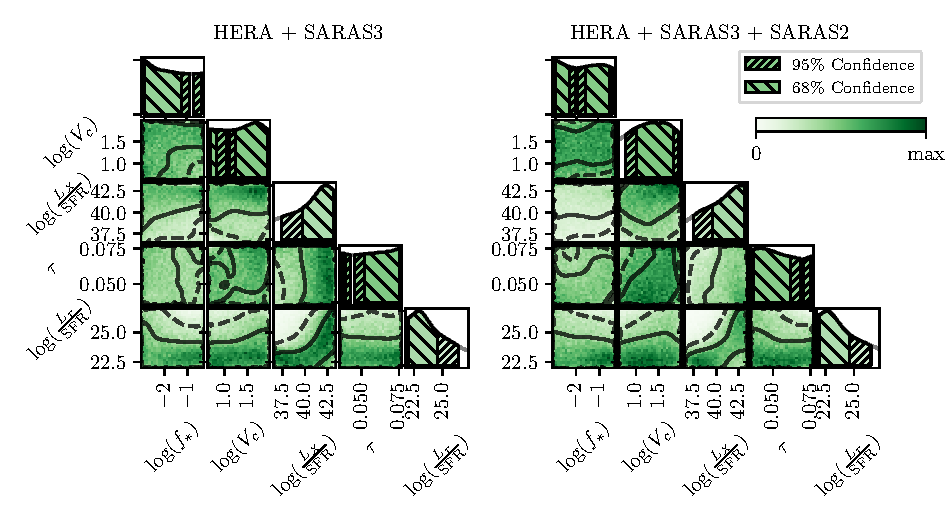
\includegraphics{joint_constraints/figs/other_global.pdf}
    \caption{\textbf{The impact of SARAS2 data on the astrophysical constraints.} We show the joint posterior distributions for HERA and SARAS3 on the left panel (identical to Figure \ref{fig:posterior}, but shown here for comparison) and for HERA, SARAS3 and SARAS2 on the right panel. SARAS2 covers the band $z\approx 7 - 12$ and therefore has some overlap with HERA but not with SARAS3. The addition of SARAS2 to the joint analysis washes out the constraint on star formation properties, $V_c$ and $f_*$, because it leads to increased uncertainty in the structure of the signals at high redshifts. However, we still see a consistent disfavouring of a population of radio galaxies with high radio and low X-ray luminosities. The one dimensional posteriors for $\tau$ appear to be in disagreement, however, we note that these are basically flat. We exclude SARAS2 from our main results in the text because of uncertainty in the modelling of systematics in the data.}
    \label{fig:other_global}
\end{figure}


\begin{figure}
    \centering
    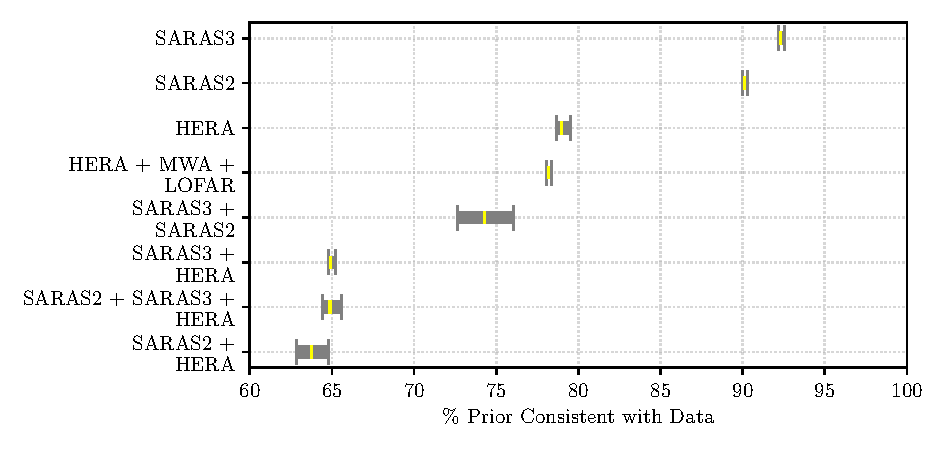
\includegraphics{joint_constraints/figs/volume_contraction.pdf}
    \caption{\textbf{Constraining power of different data sets.} The percentage of the wide astrophysical parameter prior that is found to be consistent with the different data sets and different combinations of data sets explored in this work. A lower value indicates a better set of constraints, although a difference of a few percents does not necessarily translate into significant differences in the parameter constraints, as can be seen when comparing the results from HERA and HERA + LOFAR + MWA.}
    \label{fig:volume_contraction}
\end{figure}

\subsection{Other Power Spectrum Experiments}
\label{sec:other_interferometers}

In \cref{fig:other_interferometers}, we show the projected posteriors derived using HERA data alone (left panel) and HERA, MWA and LOFAR together (right panel). We note that the constraints from the different interferometers are all at low redshifts between $z\approx 6 - 10$ and varying wavenumbers or angular scales. These are detailed in \cref{tab:interferometers} along with the constraints from the individual experiments on key parameters.

We derived parameter constraints from the MWA and LOFAR data using the approach taken in the original HERA analysis. Specifically, we take the measured upper limits, the mean power spectrum and uncertainty, and treat it as a measurement of cosmological signal plus systematics. As in HERA \cite{HERA_2022b} we take this uncertainty to be Gaussian and marginalize over a uniform prior on the systematics, yielding the likelihood
\begin{equation}
    \mathcal{L}(\theta_{21}) = \prod_i^{N_d}\frac{1}{2}\bigg(1 - \mathrm{erf}\bigg[\frac{d_i - m_i(\theta_{21})}{\sqrt{2\sigma_i}}\bigg]\bigg), 
\end{equation}
where $N_d$ represents the number of data points, $d_i$ and $\sigma_i$ correspond to the mean and standard deviation in each data point, and $m_i(\theta_{21})$ is the model prediction for that redshift and wave number. Thus, a model prediction $m\gg d$ gives $\mathcal{L}\approx0$ while $m\ll d$ gives a constant. This likelihood is effectively a step function that disfavours models above a given amplitude. A full discussion of its derivation can be found in \cite{HERA_2022b}.

We performed this joint analysis using a full analytic likelihood approach~(independent of \textsc{margarine}) since there are no nuisance parameters describing the systematics. We find that each of the experiments disfavours individually similar regions of the $L_r - L_X$ plane. However, the joint analysis does not improve the results derived from HERA data alone~(as we summarise in \cref{tab:interferometers} and is further illustrated in \cref{fig:volume_contraction}) which motivates our decision to only use HERA in the main text. 

\begin{table}[]
    \centering
    \begin{tabular}{|p{2cm}|p{3cm}|p{3cm}|p{3cm}|p{3cm}|}
        \hline
         & HERA  & LOFAR & MWA & LOFAR + MWA + HERA \\
         \hline
         $z$ & $\approx 8$ \&  $\approx 10$ & $9.1$ \&  $ 9.3 - 10.6$ & $6.5 - 8.7$ & Discrete and continuous ranges of $z$ between $6.5 - 10.6$ \\
         \hline
         $k$ [h~Mpc$^{-1}$]& $0.128 - 0.960$  & $0.075 - 0.432$ \&  $0.053$& $0.070-3.000$ & Discrete and continuous ranges of $k$ \\
         \hline
         \hline
         $L_{r}/\mathrm{SFR}$ & $\gtrsim4.00\times10^{24}$ & $\gtrsim 1.20 \times10^{25}$ & $\gtrsim1.58\times10^{25}$ & $\gtrsim4.00\times10^{24}$ \\
         \hline
         $L_{X}/\mathrm{SFR}$ & $\lesssim7.60\times10^{39}$ & $\lesssim 8.70 \times10^{38}$ & $\lesssim1.16\times10^{39}$ & $\lesssim 1.58 \times10^{40}$\\
         \hline
         $L_{r}/\mathrm{SFR}$ \&  $L_{X}/\mathrm{SFR}$ & $\gtrsim 4.00\times10^{24}$ \&  $\lesssim 7.60\times10^{39}$ & $\gtrsim 3.16\times10^{25}$ \&  $\lesssim 1.00\times10^{40}$ & $\gtrsim 1.00\times10^{25}$ \&  $\lesssim 1.00\times10^{40}$ & $\gtrsim4.00\times10^{24}$ \&  $\lesssim1.58 \times10^{40}$ \\
         \hline
    \end{tabular}
    \caption{\textbf{Constraints from interferometers.} The table shows the various constraints on the radio and X-ray luminosities for HERA, MWA, LOFAR and the combination of all three along with their respective wavenumbers and redshift ranges. The joint analysis only marginally improves our understanding of the infant universe.}
    \label{tab:interferometers}
\end{table}

\begin{figure}
    \centering
    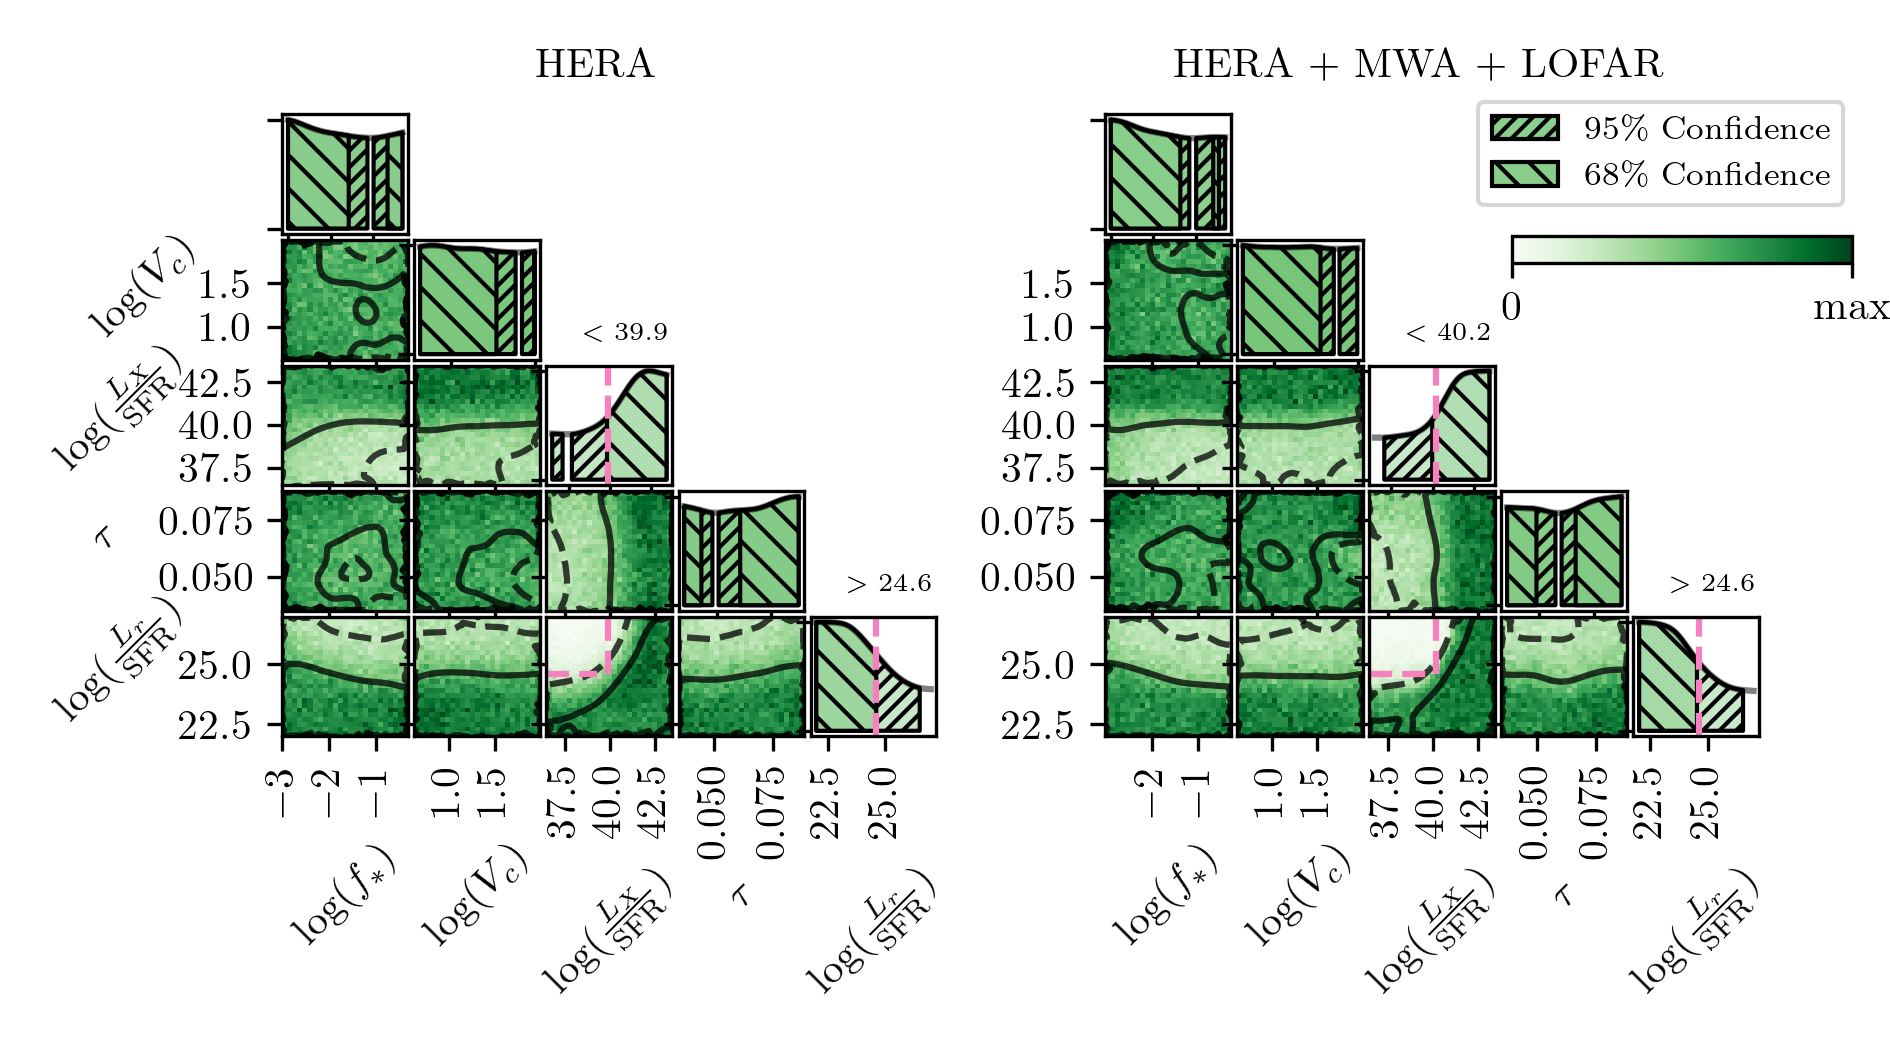
\includegraphics{joint_constraints/figs/other_interferometers.png}
    \caption{\textbf{The impact of MWA and LOFAR on the parameter constraints.} Projected posterior distribution functions (PDFs) for the 5 simulation parameters, obtained by assuming flat priors and combining different observations: HERA alone (left, as in \cite{HERA_2022b}) and LOFAR, HERA and MWA (right). Solid (dashed) lines correspond to regions containing the highest 68\% (95\%) probability. We see that HERA constraints are not significantly improved by adding the published limits on the power spectrum from other interferometers.}
    \label{fig:other_interferometers}
\end{figure}

\clearpage



















